\documentclass[runningheads]{llncs}

\usepackage[T1]{fontenc}
\usepackage{graphicx}
%\usepackage{color}
%\renewcommand\UrlFont{\color{blue}\rmfamily}

\usepackage{amsmath,amssymb,amsfonts}
\usepackage[inline, shortlabels]{enumitem}
\usepackage{tabularx}
\usepackage{caption}
\usepackage{listings}
% \usepackage{titlesec}
\usepackage[english]{babel}
\captionsetup{font=it}
\usepackage{ragged2e}
\usepackage[hyphens]{url}
\usepackage{hyperref}
\usepackage{xurl}
\usepackage{pifont}
\usepackage{footmisc}
\usepackage{multirow}
\usepackage{enumitem}
\usepackage{algorithm2e}
\usepackage{float}
\usepackage{listings}
\usepackage{xcolor}

\definecolor{codegreen}{rgb}{0,0.6,0}
\definecolor{codegray}{rgb}{0.5,0.5,0.5}
\definecolor{codepurple}{rgb}{0.58,0,0.82}
\definecolor{backcolour}{rgb}{0.95,0.95,0.92}
 
\lstdefinestyle{mystyle}{
    backgroundcolor=\color{backcolour},   
    commentstyle=\color{codegreen},
    keywordstyle=\color{magenta},
    numberstyle=\tiny\color{codegray},
    stringstyle=\color{codepurple},
    basicstyle=\footnotesize,
    breakatwhitespace=false,         
    breaklines=true,                 
    captionpos=b,                    
    keepspaces=true,                 
    numbers=left,                    
    numbersep=5pt,                  
    showspaces=false,                
    showstringspaces=false,
    showtabs=false,                  
    tabsize=2
}
 
\lstset{style=mystyle}

% --- Tickz
\usepackage{physics}
\usepackage{amsmath}
\usepackage{tikz}
\usepackage{mathdots}
\usepackage{yhmath}
\usepackage{cancel}
\usepackage{color}
\usepackage{siunitx}
\usepackage{array}
\usepackage{multirow}
\usepackage{amssymb}
\usepackage{gensymb}
\usepackage{tabularx}
\usepackage{extarrows}
\usepackage{booktabs}
\usetikzlibrary{fadings}
\usetikzlibrary{patterns}
\usetikzlibrary{shadows.blur}
\usetikzlibrary{shapes}

% ---------
% \usepackage{titlesec}
\usepackage{pdfpages}
\usepackage{booktabs}
\usepackage{csquotes}
\usepackage{lipsum}  
\usepackage{arydshln}
\usepackage{smartdiagram}
\usepackage[inkscapeformat=png]{svg}
\usepackage{textcomp}
\usepackage{tabularray}\UseTblrLibrary{varwidth}
\usepackage{xcolor}
\def\BibTeX{{\rm B\kern-.05em{\sc i\kern-.025em b}\kern-.08em
    T\kern-.1667em\lower.7ex\hbox{E}\kern-.125emX}}
\usepackage{cite}
\usepackage{amsmath}
\newcommand{\probP}{\text{I\kern-0.15em P}}
\usepackage{etoolbox}
\patchcmd{\thebibliography}{\section*{\refname}}{}{}{}

\setlength{\extrarowheight}{2.5pt}

\renewcommand{\arraystretch}{1.7}

\setlength{\extrarowheight}{2.5pt}
\renewcommand{\arraystretch}{0.2}
\renewcommand{\arraystretch}{1.7}

% --------------
% \titleclass{\subsubsubsection}{straight}[\subsection]

% \newcounter{subsubsubsection}[subsubsection]
% \renewcommand\thesubsubsubsection{\thesubsubsection.\arabic{subsubsubsection}}
% \renewcommand\theparagraph{\thesubsubsubsection.\arabic{paragraph}} % optional; useful if paragraphs are to be numbered

% \titleformat{\subsubsubsection}
%   {\normalfont\normalsize\bfseries}{\thesubsubsubsection}{1em}{}
% \titlespacing*{\subsubsubsection}
% {0pt}{3.25ex plus 1ex minus .2ex}{1.5ex plus .2ex}

% \makeatletter
% \renewcommand\paragraph{\@startsection{paragraph}{5}{\z@}%
%   {3.25ex \@plus1ex \@minus.2ex}%
%   {-1em}%
%   {\normalfont\normalsize\bfseries}}
% \renewcommand\subparagraph{\@startsection{subparagraph}{6}{\parindent}%
%   {3.25ex \@plus1ex \@minus .2ex}%
%   {-1em}%
%   {\normalfont\normalsize\bfseries}}
% \def\toclevel@subsubsubsection{4}
% \def\toclevel@paragraph{5}
% \def\toclevel@paragraph{6}
% \def\l@subsubsubsection{\@dottedtocline{4}{7em}{4em}}
% \def\l@paragraph{\@dottedtocline{5}{10em}{5em}}
% \def\l@subparagraph{\@dottedtocline{6}{14em}{6em}}
% \makeatother

% \setcounter{secnumdepth}{4}
% \setcounter{tocdepth}{4}
% --------------

\newcommand{\before}[1]{\textcolor{red}{#1}}
\newcommand{\after}[1]{\textcolor{green}{#1}}

\newcommand{\old}[1]{\textcolor{orange}{#1}}
\newcommand{\rem}[1]{\textcolor{red}{#1}}
\newcommand{\todo}[1]{\textcolor{orange}{\newline \textit{\textbf{TODO:} #1}} \newline \newline }



\newcounter{relation}
\setcounter{relation}{0}
\renewcommand{\therelation}{\arabic{relation}}
\newcommand{\relationautorefname}{Relation}

\newenvironment{relation}[1][]{%
    \refstepcounter{relation}%
    \noindent \raggedright \textit{\textbf{Relation. \therelation}} \hfill$}
{%
$ \hfill \phantom{x}

}

\newcounter{proof}
\setcounter{proof}{0}
\renewcommand{\theproof}{\arabic{proof}}
\newcommand{\proofautorefname}{Proof}

\renewenvironment{proof}[1][]{
    \refstepcounter{proof}
    \noindent \raggedright \textit{\textbf{Proof. \theproof}}

    \setlength{\leftskip}{1em}

}
{

\
\setlength{\leftskip}{0pt}
}

% --------------------------------
%             DOCUMENT
% --------------------------------

\begin{document}
\title{A MARL-based Approach for Easing MAS Organization Engineering}
%
%\titlerunning{Abbreviated paper title}
% If the paper title is too long for the running head, you can set
% an abbreviated paper title here
%
\author{Julien Soulé\inst{1}\orcidID{0000-1111-2222-3333} \and
    Jean-Paul Jamont\inst{1}\orcidID{1111-2222-3333-4444} \and
    Michel Occelo\inst{1}\orcidID{2222--3333-4444-5555} \and
    Louis-Marie Traonouez\inst{2}\orcidID{2222--3333-4444-5555} \and
    Paul Théron\inst{3}\orcidID{2222--3333-4444-5555}}
%
\authorrunning{J. Soulé et al.}
% First names are abbreviated in the running head.
% If there are more than two authors, 'et al.' is used.
%
\institute{Univ. Grenoble Alpes, Grenoble INP, LCIS, 26000, Valence, France
    \email{\{julien.soule, jean-paul.jamont, michel.occello\}@lcis.grenoble-inp.fr}
    \and
    Thales Land and Air Systems, BU IAS, Rennes, France
    \email{louis-marie.traonouez@thalesgroup.com}
    \and
    AICA IWG, La Guillermie, France \\
    \email{paul.theron@orange.fr}
}


\maketitle              % typeset the header of the contribution

% MAS have been succefully
% For many MAS, the organization has become a critical success factor. 
% Several related methods exist to design MAS. 
% However, these methods are ...
% To enhance the quality and effectiveness of ... this paper presents an assisted approach for MAS Organization Engineering (AMOEA). 
% AMOEA guides the designer of...
% 1 phrase par contrib/key point

\begin{abstract}

    % context
    Multi-Agent Systems (MAS) have been successfully applied due to their ability to address complex, distributed problems especially in IoT based systems.
    Their efficiency regarding respective objectives and requirements is strongly dependant on the organization for engineering an application-specific MAS.
    Methods to develop MAS have been proposed relying on the knowledge of the deployment environment in order to design organization that can achieve the given goals.
    % Yet, in some cases, the deployment environment is not easily readable or handleable due to the complexity and may lead to unexpected emergent phenomena raising safety concerns.
    Yet, high complexity and low readability in deployment environments may lead the application of these methods to be costly or to raise safety concerns.
    % That stresses out the need for methodological works for assisted MAS design that could be addressed with collective AI techniques.
    % hypothesis / contribution
    In order to ease the organization designing regarding those concerns, we propose an novel Assisted MAS Organization Engineering Approach (AOMEA). AOMEA relies on linking a Multi-Agent Reinforcement Learning (MARL) process with an organizational model to suggest relevant organizational specifications to help in the MAS engineering.
    % We introduce , an novel design approach to assist the MAS design whose underlying idea is to use Multi-Agent Reinforcement Learning with organizational specifications for both understanding and constraining the training process regarding design constraints.
    % results
    % We applied our approach in cooperative Atari games and a Cyberdefense drone swarm scenario of the 3rd CAGE Challenge. Obtained specifications are indeed consistent with design constraints and provide insights of relevant collective strategies that led to develop an explainable MAS with scores close to finalists' ones.

    \keywords{Multi-Agent Systems \and Organization \and Design \and Assisted engineering}
\end{abstract}

\section{Introduction}

% Context:

Multi-agent systems (MAS) have gained significant interest in engineering and industry due to their ability to address complex, distributed problems. That paradigm enables decomposing a complex task into smaller ones delegated to autonomous cooperative agents that achieve them through re/self-organization mechanisms. Most notably, they provide ways to handle conflicting goals, parallel computation, system robustness, and scalability. The applications of MAS are diverse, including collective robotics, Vehicular Ad Hoc Network (VANET), Mobile Ad Hoc Network (MANET) or Wireless Sensor Network (WSN)\cite{Oliveira1999, Gembarski2020}.
In MAS, organization is a fundamental concept that impact how agents coordinate their activities to collaboratively achieve a common goal~\cite{Hubner2002}.
Organizational aspects are crucial for addressing the challenge of MAS design in dynamic and uncertain environments, where runtime behavior needs to be flexible~\cite{Kathleen2020}. The impact organization on MAS design is core in methodologies and frameworks that enable the engineering of application-specific MAS~\cite{Bakliwal2018}.

MAS designing/development methods, have been proposed jointly with organizational models to help designers finding suited specifications of an organization so that a MAS can reach a goal efficiently in a environment. Methods such as GAIA~\cite{Wooldridge2000}, ADELFE~\cite{Bernon2003} or DIAMOND~\cite{Jamont2005} lead to develop \textbf{self/re-organization} mechanisms from agents' rules (we call \textbf{policies}) enabling the MAS to adapt on the deployment environment.
These agents' policies are defined by the designer from Agent Centered Point of View (ACPV) or Organization Centered Point of View (OCPV) so that an optional emerging/chosen organization allows reaching a global goal~\cite{Picard2009}. It often takes place as an iterative process where designers are proceeding by trial and error. Despite the designer skills, that process may be hard and costly to converge towards a sufficiently estimated successful MAS. That process gets more difficult when the target deployment environment is not easily readable or handleable due to its complexity and may raise unexpected emergent phenomena.

As an example, research in Autonomous Intelligent Cyberdefense Agents~\cite{Kott2023} (AICA) aims to develop cooperative cyber-defense agents deployed in computer networks including highly complex ones and with non-visual interactions. Additionally, the lack of intuitive comprehension of the environment can make existing MAS methods difficult to apply regarding internal safety policies such as for company infrastructure networks.

% Problem:

Instead of adopting a risky direct empiric approach, some available methodological approaches rely on a intermediary step by simulating the target deployment system, analogous to \textquote{digital twins}. Indeed, simulation can provide a monitoring framework that leaves room for a safe design process, while having an assessment of the resulting MAS designs. If the simulation is close enough to the target system in terms of fidelity, then we can expect the designed MAS to be transferred to the target system for indeed reaching the goals.

However, none of these methods provide general automated ways to guide the designing process of a MAS that has to achieve a given goal regarding the deployment environment constraints and design requirements in light of results obtained in simulation. Indeed, there is a need not only for automatically finding suited agents' policies that lead to sufficient performance which is generally done through MARL; but also to make the implicit organizational mechanisms that emerges form trained agents, explicit to the designer point of view hence enabling to consider both explainability and safety concerns in the MAS engineering.

% Contribution

In order to address that issue, we introduce AMOEA, a novel general MAS design approach whose underlying idea is to link a given MARL process with an organizational model that links the on-training agents' policies with explicit organizational specifications. It can be viewed as a tool for engineering to automatically generate relevant exploitable organizational specifications only regarding the performance in achieving the given global goal and the satisfaction of the given designer's constraints. For the designer, the obtained organizational specifications can be used as insights of the organizational mechanisms to set up during the development towards a MAS that meets performance, explainability and safety requirements.

% Results

We applied AOMEA in three spatial Atari games with various required degree of cooperation among agents so they achieve a goal the best; and additionally respecting organizational specifications as design constraints. Obtained organizational specifications are indeed exploitable, coherent with expectations, and respect design constraints.
%We also applied our approach, in a Cyberdefense drone swarm environment whose resulting organizational specifications led to develop a MAS with scores comparable to the leading ones.

Section II starts introducing the theoretical background of AOMEA as for the key role of organization in the development of a MAS and available methodological works and the motivation for integrating a MAS organizational model into a MARL process in order to enhance the MAS design process. In section III, we globally introduce AOMEA before explaining the theoretical core the approach is built on. Then, we detail how AOMEA can be applied in MAS engineering through a proposed implementation. We assessed AOMEA in 4 simulated environments discussing obtained results in section IV. Finally, section V concludes on the viability and relevance of our approach as we highlight limitations to overcome and future works as well.

% ====================================================================================================

\section{Theoretical background}

% // Mettre en avant les briques du raisonnement en expliquant le titre pour préparer l'introduction de la contribution avec AOMEA sans les justifier (sans faire de comparaison avec l'existant, pas d'édt, dire juste les points forts)

% Organization
%   -> moise (justifier parmi les existants)

% MAS methodologies (ALAADIN, GAIAI mais pas de moyens pour trouver une organisation automatiquemenet)

% MARL (basiques) // DECPOMDP (basiques)


Developing a Multi-Agent System (MAS) involves various engineering methods and methodologies that are designed to address the complexities inherent in the design, implementation, and deployment of such systems. These methods are essential for ensuring that MAS can effectively coordinate, communicate, and execute tasks in a distributed and often dynamic environment.
Several comprehensive methodologies have been proposed for MAS development, including:

\begin{itemize}
    \item \emph{Tropos}: An agent-oriented software development methodology that emphasizes early requirements analysis and the continuous refinement of these requirements through the design and implementation phases~\cite{Bresciani2004}.
    \item \emph{Gaia}: A methodology for the analysis and design of MAS, focusing on the organizational structure of the system~\cite{Zambonelli2003}.
    \item \emph{INGENIAS}: A methodology that provides a suite of tools and a formal framework for the development of MAS~\cite{Pavon2003}.
    \item \emph{MaSE (Multi-agent Systems Engineering)}: A methodology that guides the analysis and design of MAS from initial system goals to the detailed agent design~\cite{Scott2004}.
\end{itemize}

Yet, these methodological works significantly rely on human designers while none of them enable automating the assistance of the MAS design process by guaranteeing sufficient efficiency while taking into account organizational aspects in a multiagent context.

Beside, these MAS designing methods, recent works in MARL make it possible benefitting of a MARL process that would automatically converge to an optimal or sub-optimally sufficient solution as for establishing the rules in agents (called \textbf{policies}) that drive the MAS to the goal. Yet, unlike human-based design where the agent's logic is explicitly specified, trained policies with MARL may be approximated by black box generalizing functions such as Neural Networks hence not explicitly describing emergent collective strategies among trained agents.
As a recent issue, we identified few related works partially linked to using MARL for better understanding trained agents collective behavior but none are oriented for a methodological approach for MAS designing.

Kazhdan et. al.~\cite{Kazhdan2020} proposed a library to enhance the explainability of MARL systems by providing means to extract symbolic models from MARL systems. It focuses on improving the interpretability of MARL systems.
Wang et. al.~\cite{Wang2020} introduced a role-oriented MARL approach where roles are emergent, and agents with similar roles tend to share their learning and specialize in certain sub-tasks. The approach is designed to learn specialized, dynamic, and identifiable roles without relying on predefined role structures and behaviors.
Tosic et. al~\cite{Tosic2010} proposed a framework for addressing coordination in collaborative multi-agent systems. It enable agents to learn how to coordinate effectively to enhance the coordination and communication capabilities of multi-agent systems.
Zheng et. al.~\cite{Zheng2018} presented a platform for MARL that aims to facilitate research on artificial collective intelligence by providing a comprehensive set of baselines and evaluation metrics to benchmark the performance of MARL algorithms.

Our approach to address the explainability in MARL with a methodological purpose for MAS, consists in considering that a joint-policy or joint-history can be described in terms of the organizational specifications at least partially.
We refer to research in the processes falling into that broad approach under the term of \textquote{Organization oriented MARL} (OMARL).
In that context, we propose the \emph{Partial Relations with Agent History and Organization Model} (PRAHOM) process to link agents' policies and their training to an organizational model.

The chosen MARL model is based on the Decentralized Dec-POMDP~\cite{Oliehoek2016} because it considers multiple agents in a similar MAS fashion. It relies on stochastic processes to model uncertainty of the environment for the changes induced by actions, in received observations, in communication\dots Additionally, unlike Partially Observable Stochastic Games (POSG), the reward function can be common to agents which fosters training for collaborative oriented actions~\cite{Beynier2013}. Formally, a Dec-POMDP is a 7-tuple $(S,\{A_i\},T,R,\{\Omega_i\},O,\gamma)$ , where: $S = \{s_1, ..s_{|S|}\}$: The set of the possible states; $A_{i} = \{a_{1}^{i},..,a_{|A_{i}|}^{i}\}$: The set of the possible actions for agent $i$; $T$ so that $T(s,a,s') = \probP{(s'|s,a)}$ : The set of conditional transition probabilities between states; $R: S \times A \times S \rightarrow \mathbb{R}$: The reward function; $\Omega_{i} = \{o_{1}^{i},..,o_{|\Omega_{i}|}^{i}\}$: The set of observations for agent $ag_i$; $O$ so that $O(s',a,o) = \probP{(o|s',a)}$ : The set of conditional observation probabilities; $\gamma \in [0,1]$, the discount factor.

Among, the existing organizational models \textquote{Agent/Group/Role}~\cite{Ferber2004} and \allowbreak $\mathcal{M}OISE^+$~\cite{Hubner2002} both provide a relevant high-level description of the structures and interactions within the MAS. However, we favor $\mathcal{M}OISE^+$ because it provides an advanced formal description for an organization without incompatibilities with MARL, especially for formal description of agents' policies. It takes into account explicitly the social aspects between agents where \textquote{AGR} focuses on the integration of standards oriented towards design. Additionally, it provides a sufficiently detailed vision of organization to be understood at different point of views. $\mathcal{M}OISE^+$ comprises: Structural specifications mainly related to roles, their links, compatibilities\dots; Functional specifications mainly related to goals, their repartition in missions and plans\dots; Deontic Specifications as the permission and obligations for a agent playing a role to commit to a mission~\cite{Hubner2002}.



% ====
% \paragraph{\textbf{Method Fragments and Model Transformations}}
% A set of method fragments for developing MAS, which is grounded on the development process of two multi-agent systems, emphasizes the importance of model transformations in the engineering process~\cite{Garcia2011}. These fragments can be seen as modular methodologies that can be adapted and reused across different MAS projects, providing a flexible approach to system development.

% \paragraph{\textbf{Meta-Models for Analysis and Design}}
% The use of meta-models is reported to improve analysis and design activities in MAS engineering~\cite{Gomez2004}. Meta-models provide a high-level abstraction that can help in understanding and designing the complex interactions and behaviors of agents within the system, facilitating a more structured approach to MAS development.

% \paragraph{\textbf{Agent-Oriented Software Engineering Paradigms}}

% Agent technology represents a new software engineering paradigm that offers fresh prospects for analyzing, designing, and building software systems~\cite{Li2016}. This paradigm shift towards agent-oriented software engineering (AOSE) encourages developers to think in terms of autonomous agents and their interactions, leading to more robust and adaptable MAS.

% \paragraph{\textbf{Comprehensive Methodologies}}

% \paragraph{\textbf{Characterization of emergent collective strategies}}

% % Collective explainable AI: Explaining cooperative strategies and agent contribution in multiagent reinforcement learning with shapley values
% Heuillet et. al.~\cite{Heuillet2022} proposes a novel approach to explain cooperative strategies in multiagent reinforcement learning (RL) using Shapley values, a game theory concept used in eXplainable AI (XAI). The study aims to make deep RL more comprehensible and address the need for methods that provide better understanding and interpretability. The experimental results on Multiagent Particle and Sequential Social Dilemmas demonstrate the effectiveness of Shapley values in explaining the rationale behind decisions taken by agents. However, the article also highlights that Shapley values can only provide general explanations about a model and cannot explain specific actions taken by agents. The authors suggest that future work should focus on addressing these limitations. The study's implications extend to areas such as non-discriminatory decision making, ethical and responsible AI-derived decisions, and policy making under fairness constraints.

% % Social Influence as Intrinsic Motivation for Multi-Agent Deep Reinforcement Learning
% Jaques et. al.~\cite{Jaques2019} proposes a mechanism for achieving coordination and communication in MARL by rewarding agents for having causal influence over other agents' actions. This causal influence is assessed using counterfactual reasoning, where agents simulate alternate actions to compute their effect on the behavior of other agents. The paper demonstrates that this approach leads to enhanced coordination and communication, as well as more meaningful learned communication protocols. The proposed method is shown to significantly increase the learning curves of the deep reinforcement learning agents, leading to more diversified team behavior and more successful performance of the population as a whole. The paper also highlights that the influence rewards for all agents can be computed in a decentralized way, opening up new opportunities for research in this area.

% \paragraph{\textbf{Adaptation of MARL to meet requirements}}

% % Efficient MARL through automated supervision
% Chongjie et. al.~\cite{Chongjie2008} proposes a unified mechanism for achieving coordination and communication in MARL. The approach involves training multiple agents to independently maximize their own individual reward without sharing weights. The paper introduces a method for automated supervision, which enables the agents to learn to coordinate and communicate effectively. This automated supervision mechanism leads to enhanced coordination, communication, and more meaningful learned communication protocols, ultimately improving the learning curves of the deep reinforcement learning agents and the overall performance of the agent population
% %
% % Self-Organized Group for Cooperative MARL
% Shao et. al.~\cite{Shao2022} introduces a method called Self-Organized Group (SOG) for cooperative MARL. In this approach, a certain number of agents are randomly elected to be conductors, and the corresponding groups are constructed with conductor-follower consensus, allowing the groups to be re-organized at regular intervals. The organized group under the unified command of a conductor is found to embed the multi-agent system with stronger zero-shot generalization ability compared to traditional methods. The SOG method provides strong adaptability to scenarios with varying numbers of agents and varying agent sight. The paper presents this approach as a mechanism to enhance cooperative multi-agent tasks with dynamic characteristics, aiming to improve the adaptability and generalization of MARL systems
%
% % A MARL model of common-pool resource appropriation
% Perolat et. al.~\cite{Perolat2017} introduces a model that focuses on common-pool resource appropriation, a multi-agent social dilemma that includes issues such as sustainable use of fresh water, common fisheries, grazing pastures, and irrigation systems. The model emphasizes the importance of trial-and-error learning in addressing the challenges of common-pool resource sustainability and inequality. It explores the emergent behavior of groups of independently learning agents in a partially observed Markov game, shedding light on the relationship between exclusion, cooperation, and sustainability in the context of resource appropriation. The research highlights the potential of deep reinforcement learning in understanding and addressing complex societal and environmental challenges related to common-pool resource management. The paper provides valuable insights into the application of MARL in the context of real-world social dilemmas and resource management
%
% Promoting Coordination through Policy Regularization in Multi-Agent Deep Reinforcement Learning
% Roy et. al.~\cite{Roy2020} addresses the challenge of inducing coordination between agents in MARL. The research investigates the use of policy regularization to promote inter-agent coordination and discusses two approaches based on inter-agent modeling and synchronized sub-policy selection. The proposed methods are designed to improve cooperative behaviors without relying on explicit communication channels, allowing agents to exhibit coordinated behaviors during testing when acting in a decentralized fashion. The paper presents two policy regularization methods, TeamReg and CoachReg, and evaluates their performance on challenging cooperative multi-agent problems, showing improved results. The research contributes to the advancement of coordination-driven multi-agent approaches in reinforcement learning and provides valuable insights into promoting inter-agent coordination through policy regularization.

% Eventually, among considered works, none are specifically using an organizational model as a general way for both expressing the MARL resulting through OCPV; and constraining the MARL itself according to organizational specifications. It appears that augmenting MARL with an organizational model so it can be core of a aided-engineering MAS design approach; is not explicitly covered as far as we know.

% ====================================================================================================

\section{AOMEA approach}

% Mettre d'abord en avant le shcéma général de l'approche
% Donner la philosophie de l'approche


% TODO: The Assisted Organization...

% AOMEA approach

% TODO: confirmer les choix faits en "theortecial background" vis à vis du problème

% 	Global overview (Fig 1)
% 	theoreetical core
% 	Engineering
%   Implémentation (vers une implémentation de type PoC)

\section{Global overview}

\begin{figure}[t!]
    \centering
    


\tikzset{every picture/.style={line width=0.75pt}} %set default line width to 0.75pt        

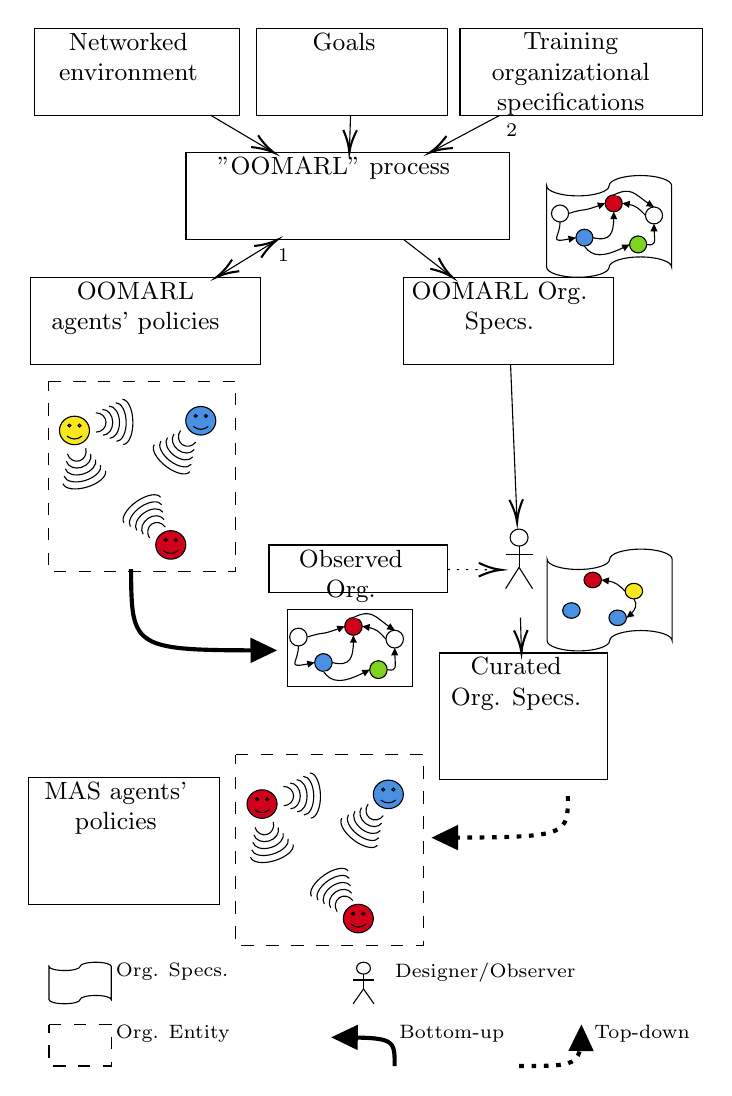
\begin{tikzpicture}[x=0.75pt,y=0.75pt,yscale=-1,xscale=1]
%uncomment if require: \path (0,567); %set diagram left start at 0, and has height of 567

%Flowchart: Punched Tape [id:dp6253416173354658] 
\draw  [fill={rgb, 255:red, 255; green, 255; blue, 255 }  ,fill opacity=1 ] (250,275.87) .. controls (250,278.58) and (256.74,280.77) .. (265.06,280.77) .. controls (273.38,280.77) and (280.12,278.58) .. (280.12,275.87) .. controls (280.12,273.16) and (286.87,270.97) .. (295.18,270.97) .. controls (303.5,270.97) and (310.25,273.16) .. (310.25,275.87) -- (310.25,315.1) .. controls (310.25,312.39) and (303.5,310.19) .. (295.18,310.19) .. controls (286.87,310.19) and (280.12,312.39) .. (280.12,315.1) .. controls (280.12,317.8) and (273.38,320) .. (265.06,320) .. controls (256.74,320) and (250,317.8) .. (250,315.1) -- cycle ;
%Shape: Ellipse [id:dp3141849675822821] 
\draw  [fill={rgb, 255:red, 208; green, 2; blue, 27 }  ,fill opacity=1 ] (267.77,285.83) .. controls (267.77,283.76) and (269.66,282.08) .. (271.98,282.08) .. controls (274.3,282.08) and (276.19,283.76) .. (276.19,285.83) .. controls (276.19,287.9) and (274.3,289.58) .. (271.98,289.58) .. controls (269.66,289.58) and (267.77,287.9) .. (267.77,285.83) -- cycle ;
%Shape: Ellipse [id:dp24618456488955864] 
\draw  [fill={rgb, 255:red, 248; green, 231; blue, 28 }  ,fill opacity=1 ] (287.6,291.19) .. controls (287.6,289.12) and (289.49,287.44) .. (291.81,287.44) .. controls (294.13,287.44) and (296.02,289.12) .. (296.02,291.19) .. controls (296.02,293.27) and (294.13,294.95) .. (291.81,294.95) .. controls (289.49,294.95) and (287.6,293.27) .. (287.6,291.19) -- cycle ;
%Shape: Ellipse [id:dp8783844186516785] 
\draw  [fill={rgb, 255:red, 74; green, 144; blue, 226 }  ,fill opacity=1 ] (279.79,304.06) .. controls (279.79,301.99) and (281.67,300.31) .. (284,300.31) .. controls (286.32,300.31) and (288.2,301.99) .. (288.2,304.06) .. controls (288.2,306.13) and (286.32,307.81) .. (284,307.81) .. controls (281.67,307.81) and (279.79,306.13) .. (279.79,304.06) -- cycle ;
%Curve Lines [id:da8862512396754962] 
\draw [fill={rgb, 255:red, 255; green, 255; blue, 255 }  ,fill opacity=1 ]   (287.6,291.19) .. controls (284.11,287.9) and (283.1,286.97) .. (279.08,286.26) ;
\draw [shift={(276.19,285.83)}, rotate = 7.39] [fill={rgb, 255:red, 0; green, 0; blue, 0 }  ][line width=0.08]  [draw opacity=0] (3.57,-1.72) -- (0,0) -- (3.57,1.72) -- cycle    ;
%Shape: Ellipse [id:dp10865415349748586] 
\draw  [fill={rgb, 255:red, 74; green, 144; blue, 226 }  ,fill opacity=1 ] (257.5,300.55) .. controls (257.5,298.48) and (259.38,296.8) .. (261.71,296.8) .. controls (264.03,296.8) and (265.91,298.48) .. (265.91,300.55) .. controls (265.91,302.62) and (264.03,304.3) .. (261.71,304.3) .. controls (259.38,304.3) and (257.5,302.62) .. (257.5,300.55) -- cycle ;
%Curve Lines [id:da9209146587835657] 
\draw [fill={rgb, 255:red, 255; green, 255; blue, 255 }  ,fill opacity=1 ]   (291.81,294.95) .. controls (293.69,297.65) and (292.57,300.02) .. (290.45,302.13) ;
\draw [shift={(288.2,304.06)}, rotate = 322.38] [fill={rgb, 255:red, 0; green, 0; blue, 0 }  ][line width=0.08]  [draw opacity=0] (3.57,-1.72) -- (0,0) -- (3.57,1.72) -- cycle    ;

%Shape: Rectangle [id:dp5799704037482001] 
\draw  [dash pattern={on 4.5pt off 4.5pt}] (9.63,190) -- (100,190) -- (100,281.94) -- (9.63,281.94) -- cycle ;
%Shape: Smiley Face [id:dp642715493380654] 
\draw  [fill={rgb, 255:red, 248; green, 231; blue, 28 }  ,fill opacity=1 ] (15.05,213.78) .. controls (15.05,209.99) and (18.29,206.92) .. (22.28,206.92) .. controls (26.28,206.92) and (29.51,209.99) .. (29.51,213.78) .. controls (29.51,217.57) and (26.28,220.65) .. (22.28,220.65) .. controls (18.29,220.65) and (15.05,217.57) .. (15.05,213.78) -- cycle ; \draw  [fill={rgb, 255:red, 248; green, 231; blue, 28 }  ,fill opacity=1 ] (19.1,211.45) .. controls (19.1,211.07) and (19.43,210.76) .. (19.82,210.76) .. controls (20.22,210.76) and (20.55,211.07) .. (20.55,211.45) .. controls (20.55,211.83) and (20.22,212.13) .. (19.82,212.13) .. controls (19.43,212.13) and (19.1,211.83) .. (19.1,211.45) -- cycle ; \draw  [fill={rgb, 255:red, 248; green, 231; blue, 28 }  ,fill opacity=1 ] (24.02,211.45) .. controls (24.02,211.07) and (24.34,210.76) .. (24.74,210.76) .. controls (25.14,210.76) and (25.46,211.07) .. (25.46,211.45) .. controls (25.46,211.83) and (25.14,212.13) .. (24.74,212.13) .. controls (24.34,212.13) and (24.02,211.83) .. (24.02,211.45) -- cycle ; \draw   (18.67,216.53) .. controls (21.08,218.36) and (23.49,218.36) .. (25.9,216.53) ;
%Shape: Arc [id:dp7103754459108031] 
\draw  [draw opacity=0] (37.24,233.21) .. controls (37.24,233.21) and (37.24,233.21) .. (37.24,233.21) .. controls (38,235.82) and (34.04,239.33) .. (28.39,241.04) .. controls (22.74,242.76) and (17.53,242.04) .. (16.77,239.43) -- (27,236.32) -- cycle ; \draw   (37.24,233.21) .. controls (37.24,233.21) and (37.24,233.21) .. (37.24,233.21) .. controls (38,235.82) and (34.04,239.33) .. (28.39,241.04) .. controls (22.74,242.76) and (17.53,242.04) .. (16.77,239.43) ;  
%Shape: Arc [id:dp9993647702991559] 
\draw  [draw opacity=0] (34.85,230.5) .. controls (35.62,233.11) and (32.31,236.42) .. (27.46,237.89) .. controls (22.62,239.37) and (18.07,238.44) .. (17.3,235.83) -- (26.08,233.17) -- cycle ; \draw   (34.85,230.5) .. controls (35.62,233.11) and (32.31,236.42) .. (27.46,237.89) .. controls (22.62,239.37) and (18.07,238.44) .. (17.3,235.83) ;  
%Shape: Arc [id:dp33021260729129986] 
\draw  [draw opacity=0] (32.46,227.79) .. controls (32.46,227.79) and (32.46,227.79) .. (32.46,227.79) .. controls (32.46,227.79) and (32.46,227.79) .. (32.46,227.79) .. controls (33.23,230.4) and (30.58,233.51) .. (26.54,234.74) .. controls (22.5,235.97) and (18.61,234.85) .. (17.84,232.24) -- (25.15,230.02) -- cycle ; \draw   (32.46,227.79) .. controls (32.46,227.79) and (32.46,227.79) .. (32.46,227.79) .. controls (32.46,227.79) and (32.46,227.79) .. (32.46,227.79) .. controls (33.23,230.4) and (30.58,233.51) .. (26.54,234.74) .. controls (22.5,235.97) and (18.61,234.85) .. (17.84,232.24) ;  
%Shape: Arc [id:dp7515950702187679] 
\draw  [draw opacity=0] (30.07,225.09) .. controls (30.07,225.09) and (30.07,225.09) .. (30.07,225.09) .. controls (30.07,225.09) and (30.07,225.09) .. (30.07,225.09) .. controls (30.84,227.7) and (28.84,230.61) .. (25.61,231.59) .. controls (22.38,232.57) and (19.14,231.25) .. (18.38,228.64) -- (24.22,226.86) -- cycle ; \draw   (30.07,225.09) .. controls (30.07,225.09) and (30.07,225.09) .. (30.07,225.09) .. controls (30.07,225.09) and (30.07,225.09) .. (30.07,225.09) .. controls (30.84,227.7) and (28.84,230.61) .. (25.61,231.59) .. controls (22.38,232.57) and (19.14,231.25) .. (18.38,228.64) ;  
%Shape: Arc [id:dp17995425823285305] 
\draw  [draw opacity=0] (27.69,222.38) .. controls (27.69,222.38) and (27.69,222.38) .. (27.69,222.38) .. controls (27.69,222.38) and (27.69,222.38) .. (27.69,222.38) .. controls (28.45,224.99) and (27.11,227.7) .. (24.69,228.44) .. controls (22.27,229.18) and (19.68,227.66) .. (18.91,225.05) -- (23.3,223.71) -- cycle ; \draw   (27.69,222.38) .. controls (27.69,222.38) and (27.69,222.38) .. (27.69,222.38) .. controls (27.69,222.38) and (27.69,222.38) .. (27.69,222.38) .. controls (28.45,224.99) and (27.11,227.7) .. (24.69,228.44) .. controls (22.27,229.18) and (19.68,227.66) .. (18.91,225.05) ;  

%Shape: Arc [id:dp8934563741256025] 
\draw  [draw opacity=0] (45.36,198.82) .. controls (48.04,198.76) and (50.3,203.58) .. (50.42,209.59) .. controls (50.54,215.59) and (48.46,220.49) .. (45.78,220.55) -- (45.57,209.68) -- cycle ; \draw   (45.36,198.82) .. controls (48.04,198.76) and (50.3,203.58) .. (50.42,209.59) .. controls (50.54,215.59) and (48.46,220.49) .. (45.78,220.55) ;  
%Shape: Arc [id:dp5963815446588989] 
\draw  [draw opacity=0] (42.16,200.43) .. controls (44.84,200.38) and (47.09,204.51) .. (47.19,209.65) .. controls (47.29,214.79) and (45.2,219.01) .. (42.52,219.06) -- (42.34,209.75) -- cycle ; \draw   (42.16,200.43) .. controls (44.84,200.38) and (47.09,204.51) .. (47.19,209.65) .. controls (47.29,214.79) and (45.2,219.01) .. (42.52,219.06) ;  
%Shape: Arc [id:dp3378668028957823] 
\draw  [draw opacity=0] (38.96,202.05) .. controls (38.96,202.05) and (38.96,202.05) .. (38.96,202.05) .. controls (38.96,202.05) and (38.96,202.05) .. (38.96,202.05) .. controls (41.63,202) and (43.87,205.43) .. (43.96,209.71) .. controls (44.04,214) and (41.94,217.52) .. (39.26,217.57) -- (39.11,209.81) -- cycle ; \draw   (38.96,202.05) .. controls (38.96,202.05) and (38.96,202.05) .. (38.96,202.05) .. controls (38.96,202.05) and (38.96,202.05) .. (38.96,202.05) .. controls (41.63,202) and (43.87,205.43) .. (43.96,209.71) .. controls (44.04,214) and (41.94,217.52) .. (39.26,217.57) ;  
%Shape: Arc [id:dp7870035207223711] 
\draw  [draw opacity=0] (35.76,203.67) .. controls (38.43,203.61) and (40.66,206.35) .. (40.72,209.78) .. controls (40.79,213.21) and (38.67,216.03) .. (36,216.09) -- (35.88,209.88) -- cycle ; \draw   (35.76,203.67) .. controls (38.43,203.61) and (40.66,206.35) .. (40.72,209.78) .. controls (40.79,213.21) and (38.67,216.03) .. (36,216.09) ;  
%Shape: Arc [id:dp7731275981870975] 
\draw  [draw opacity=0] (32.55,205.29) .. controls (32.55,205.29) and (32.55,205.29) .. (32.55,205.29) .. controls (35.23,205.23) and (37.44,207.27) .. (37.49,209.84) .. controls (37.54,212.42) and (35.41,214.54) .. (32.73,214.6) -- (32.64,209.94) -- cycle ; \draw   (32.55,205.29) .. controls (32.55,205.29) and (32.55,205.29) .. (32.55,205.29) .. controls (35.23,205.23) and (37.44,207.27) .. (37.49,209.84) .. controls (37.54,212.42) and (35.41,214.54) .. (32.73,214.6) ;  

%Shape: Smiley Face [id:dp8522771230099253] 
\draw  [fill={rgb, 255:red, 208; green, 2; blue, 27 }  ,fill opacity=1 ] (61.44,268.94) .. controls (61.44,265.15) and (64.68,262.08) .. (68.67,262.08) .. controls (72.66,262.08) and (75.9,265.15) .. (75.9,268.94) .. controls (75.9,272.73) and (72.66,275.81) .. (68.67,275.81) .. controls (64.68,275.81) and (61.44,272.73) .. (61.44,268.94) -- cycle ; \draw  [fill={rgb, 255:red, 208; green, 2; blue, 27 }  ,fill opacity=1 ] (65.49,266.61) .. controls (65.49,266.23) and (65.81,265.92) .. (66.21,265.92) .. controls (66.61,265.92) and (66.94,266.23) .. (66.94,266.61) .. controls (66.94,266.99) and (66.61,267.29) .. (66.21,267.29) .. controls (65.81,267.29) and (65.49,266.99) .. (65.49,266.61) -- cycle ; \draw  [fill={rgb, 255:red, 208; green, 2; blue, 27 }  ,fill opacity=1 ] (70.41,266.61) .. controls (70.41,266.23) and (70.73,265.92) .. (71.13,265.92) .. controls (71.53,265.92) and (71.85,266.23) .. (71.85,266.61) .. controls (71.85,266.99) and (71.53,267.29) .. (71.13,267.29) .. controls (70.73,267.29) and (70.41,266.99) .. (70.41,266.61) -- cycle ; \draw   (65.06,271.69) .. controls (67.47,273.52) and (69.88,273.52) .. (72.29,271.69) ;
%Shape: Arc [id:dp2662505393390908] 
\draw  [draw opacity=0] (46.11,258.27) .. controls (46.11,258.27) and (46.11,258.27) .. (46.11,258.27) .. controls (46.11,258.27) and (46.11,258.27) .. (46.11,258.27) .. controls (44.6,256.02) and (47.31,251.45) .. (52.18,248.06) .. controls (57.04,244.66) and (62.22,243.73) .. (63.73,245.98) -- (54.92,252.13) -- cycle ; \draw   (46.11,258.27) .. controls (46.11,258.27) and (46.11,258.27) .. (46.11,258.27) .. controls (46.11,258.27) and (46.11,258.27) .. (46.11,258.27) .. controls (44.6,256.02) and (47.31,251.45) .. (52.18,248.06) .. controls (57.04,244.66) and (62.22,243.73) .. (63.73,245.98) ;  
%Shape: Arc [id:dp5533657200850002] 
\draw  [draw opacity=0] (49.2,260.11) .. controls (49.2,260.11) and (49.2,260.11) .. (49.2,260.11) .. controls (47.68,257.86) and (49.84,253.68) .. (54.01,250.77) .. controls (58.18,247.86) and (62.79,247.32) .. (64.3,249.57) -- (56.75,254.84) -- cycle ; \draw   (49.2,260.11) .. controls (49.2,260.11) and (49.2,260.11) .. (49.2,260.11) .. controls (47.68,257.86) and (49.84,253.68) .. (54.01,250.77) .. controls (58.18,247.86) and (62.79,247.32) .. (64.3,249.57) ;  
%Shape: Arc [id:dp130720604660594] 
\draw  [draw opacity=0] (52.28,261.94) .. controls (50.77,259.69) and (52.36,255.91) .. (55.84,253.48) .. controls (59.31,251.06) and (63.36,250.91) .. (64.87,253.16) -- (58.58,257.55) -- cycle ; \draw   (52.28,261.94) .. controls (50.77,259.69) and (52.36,255.91) .. (55.84,253.48) .. controls (59.31,251.06) and (63.36,250.91) .. (64.87,253.16) ;  
%Shape: Arc [id:dp7777326608896638] 
\draw  [draw opacity=0] (55.37,263.77) .. controls (55.37,263.77) and (55.37,263.77) .. (55.37,263.77) .. controls (53.86,261.53) and (54.88,258.13) .. (57.66,256.19) .. controls (60.44,254.25) and (63.93,254.5) .. (65.44,256.75) -- (60.41,260.26) -- cycle ; \draw   (55.37,263.77) .. controls (55.37,263.77) and (55.37,263.77) .. (55.37,263.77) .. controls (53.86,261.53) and (54.88,258.13) .. (57.66,256.19) .. controls (60.44,254.25) and (63.93,254.5) .. (65.44,256.75) ;  
%Shape: Arc [id:dp4348101062357661] 
\draw  [draw opacity=0] (58.46,265.61) .. controls (56.94,263.36) and (57.41,260.36) .. (59.49,258.91) .. controls (61.58,257.45) and (64.49,258.09) .. (66.01,260.34) -- (62.23,262.98) -- cycle ; \draw   (58.46,265.61) .. controls (56.94,263.36) and (57.41,260.36) .. (59.49,258.91) .. controls (61.58,257.45) and (64.49,258.09) .. (66.01,260.34) ;  

%Shape: Smiley Face [id:dp8996964185972032] 
\draw  [fill={rgb, 255:red, 74; green, 144; blue, 226 }  ,fill opacity=1 ] (75.9,209.12) .. controls (75.9,205.33) and (79.14,202.26) .. (83.13,202.26) .. controls (87.12,202.26) and (90.36,205.33) .. (90.36,209.12) .. controls (90.36,212.91) and (87.12,215.99) .. (83.13,215.99) .. controls (79.14,215.99) and (75.9,212.91) .. (75.9,209.12) -- cycle ; \draw  [fill={rgb, 255:red, 74; green, 144; blue, 226 }  ,fill opacity=1 ] (79.95,206.79) .. controls (79.95,206.41) and (80.27,206.1) .. (80.67,206.1) .. controls (81.07,206.1) and (81.4,206.41) .. (81.4,206.79) .. controls (81.4,207.17) and (81.07,207.48) .. (80.67,207.48) .. controls (80.27,207.48) and (79.95,207.17) .. (79.95,206.79) -- cycle ; \draw  [fill={rgb, 255:red, 74; green, 144; blue, 226 }  ,fill opacity=1 ] (84.87,206.79) .. controls (84.87,206.41) and (85.19,206.1) .. (85.59,206.1) .. controls (85.99,206.1) and (86.31,206.41) .. (86.31,206.79) .. controls (86.31,207.17) and (85.99,207.48) .. (85.59,207.48) .. controls (85.19,207.48) and (84.87,207.17) .. (84.87,206.79) -- cycle ; \draw   (79.52,211.87) .. controls (81.93,213.7) and (84.34,213.7) .. (86.75,211.87) ;
%Shape: Arc [id:dp6344973920370733] 
\draw  [draw opacity=0] (77.83,233.64) .. controls (77.83,233.64) and (77.83,233.64) .. (77.83,233.64) .. controls (76.23,235.82) and (71.1,234.67) .. (66.38,231.07) .. controls (61.66,227.47) and (59.13,222.79) .. (60.74,220.61) -- (69.28,227.13) -- cycle ; \draw   (77.83,233.64) .. controls (77.83,233.64) and (77.83,233.64) .. (77.83,233.64) .. controls (76.23,235.82) and (71.1,234.67) .. (66.38,231.07) .. controls (61.66,227.47) and (59.13,222.79) .. (60.74,220.61) ;  
%Shape: Arc [id:dp2502725185770005] 
\draw  [draw opacity=0] (78.55,230.08) .. controls (78.55,230.08) and (78.55,230.08) .. (78.55,230.08) .. controls (78.55,230.08) and (78.55,230.08) .. (78.55,230.08) .. controls (76.94,232.26) and (72.36,231.53) .. (68.31,228.44) .. controls (64.27,225.36) and (62.29,221.09) .. (63.9,218.91) -- (71.22,224.49) -- cycle ; \draw   (78.55,230.08) .. controls (78.55,230.08) and (78.55,230.08) .. (78.55,230.08) .. controls (78.55,230.08) and (78.55,230.08) .. (78.55,230.08) .. controls (76.94,232.26) and (72.36,231.53) .. (68.31,228.44) .. controls (64.27,225.36) and (62.29,221.09) .. (63.9,218.91) ;  
%Shape: Arc [id:dp23421846029392612] 
\draw  [draw opacity=0] (79.27,226.52) .. controls (79.27,226.52) and (79.27,226.52) .. (79.27,226.52) .. controls (79.27,226.52) and (79.27,226.52) .. (79.27,226.52) .. controls (77.66,228.7) and (73.63,228.38) .. (70.25,225.81) .. controls (66.88,223.24) and (65.45,219.39) .. (67.06,217.21) -- (73.16,221.86) -- cycle ; \draw   (79.27,226.52) .. controls (79.27,226.52) and (79.27,226.52) .. (79.27,226.52) .. controls (79.27,226.52) and (79.27,226.52) .. (79.27,226.52) .. controls (77.66,228.7) and (73.63,228.38) .. (70.25,225.81) .. controls (66.88,223.24) and (65.45,219.39) .. (67.06,217.21) ;  
%Shape: Arc [id:dp02946644855410807] 
\draw  [draw opacity=0] (79.98,222.95) .. controls (78.38,225.13) and (74.89,225.23) .. (72.19,223.18) .. controls (69.49,221.12) and (68.61,217.69) .. (70.22,215.51) -- (75.1,219.23) -- cycle ; \draw   (79.98,222.95) .. controls (78.38,225.13) and (74.89,225.23) .. (72.19,223.18) .. controls (69.49,221.12) and (68.61,217.69) .. (70.22,215.51) ;  
%Shape: Arc [id:dp07919277634076938] 
\draw  [draw opacity=0] (80.7,219.39) .. controls (80.7,219.39) and (80.7,219.39) .. (80.7,219.39) .. controls (79.1,221.57) and (76.15,222.09) .. (74.13,220.55) .. controls (72.11,219) and (71.77,215.99) .. (73.38,213.81) -- (77.04,216.6) -- cycle ; \draw   (80.7,219.39) .. controls (80.7,219.39) and (80.7,219.39) .. (80.7,219.39) .. controls (79.1,221.57) and (76.15,222.09) .. (74.13,220.55) .. controls (72.11,219) and (71.77,215.99) .. (73.38,213.81) ;  

%Flowchart: Punched Tape [id:dp1596519476860545] 
\draw  [fill={rgb, 255:red, 255; green, 255; blue, 255 }  ,fill opacity=1 ] (249.75,95.87) .. controls (249.75,98.58) and (256.5,100.77) .. (264.82,100.77) .. controls (273.13,100.77) and (279.88,98.58) .. (279.88,95.87) .. controls (279.88,93.16) and (286.62,90.97) .. (294.94,90.97) .. controls (303.26,90.97) and (310,93.16) .. (310,95.87) -- (310,135.1) .. controls (310,132.39) and (303.26,130.19) .. (294.94,130.19) .. controls (286.62,130.19) and (279.88,132.39) .. (279.88,135.1) .. controls (279.88,137.8) and (273.13,140) .. (264.82,140) .. controls (256.5,140) and (249.75,137.8) .. (249.75,135.1) -- cycle ;
%Shape: Ellipse [id:dp002685494295735058] 
\draw  [fill={rgb, 255:red, 255; green, 255; blue, 255 }  ,fill opacity=1 ] (252.11,109.26) .. controls (252.11,107.01) and (253.95,105.18) .. (256.22,105.18) .. controls (258.5,105.18) and (260.34,107.01) .. (260.34,109.26) .. controls (260.34,111.51) and (258.5,113.33) .. (256.22,113.33) .. controls (253.95,113.33) and (252.11,111.51) .. (252.11,109.26) -- cycle ;
%Shape: Ellipse [id:dp18321883985201803] 
\draw  [fill={rgb, 255:red, 74; green, 144; blue, 226 }  ,fill opacity=1 ] (263.87,120.91) .. controls (263.87,118.65) and (265.71,116.83) .. (267.98,116.83) .. controls (270.26,116.83) and (272.1,118.65) .. (272.1,120.91) .. controls (272.1,123.16) and (270.26,124.98) .. (267.98,124.98) .. controls (265.71,124.98) and (263.87,123.16) .. (263.87,120.91) -- cycle ;
%Shape: Ellipse [id:dp4076602785297232] 
\draw  [fill={rgb, 255:red, 208; green, 2; blue, 27 }  ,fill opacity=1 ] (277.98,104.36) .. controls (277.98,102.11) and (279.82,100.29) .. (282.1,100.29) .. controls (284.37,100.29) and (286.21,102.11) .. (286.21,104.36) .. controls (286.21,106.62) and (284.37,108.44) .. (282.1,108.44) .. controls (279.82,108.44) and (277.98,106.62) .. (277.98,104.36) -- cycle ;
%Shape: Ellipse [id:dp9213295790384606] 
\draw  [fill={rgb, 255:red, 255; green, 255; blue, 255 }  ,fill opacity=1 ] (297.38,110.19) .. controls (297.38,107.94) and (299.23,106.11) .. (301.5,106.11) .. controls (303.77,106.11) and (305.62,107.94) .. (305.62,110.19) .. controls (305.62,112.44) and (303.77,114.27) .. (301.5,114.27) .. controls (299.23,114.27) and (297.38,112.44) .. (297.38,110.19) -- cycle ;
%Shape: Ellipse [id:dp07303077783269196] 
\draw  [fill={rgb, 255:red, 126; green, 211; blue, 33 }  ,fill opacity=1 ] (289.74,124.17) .. controls (289.74,121.92) and (291.58,120.09) .. (293.86,120.09) .. controls (296.13,120.09) and (297.97,121.92) .. (297.97,124.17) .. controls (297.97,126.42) and (296.13,128.24) .. (293.86,128.24) .. controls (291.58,128.24) and (289.74,126.42) .. (289.74,124.17) -- cycle ;
%Curve Lines [id:da40084119138850793] 
\draw [fill={rgb, 255:red, 255; green, 255; blue, 255 }  ,fill opacity=1 ]   (260.34,109.26) .. controls (269.59,106.35) and (265.25,108.92) .. (275.25,105.36) ;
\draw [shift={(277.98,104.36)}, rotate = 159.68] [fill={rgb, 255:red, 0; green, 0; blue, 0 }  ][line width=0.08]  [draw opacity=0] (3.57,-1.72) -- (0,0) -- (3.57,1.72) -- cycle    ;
%Curve Lines [id:da056316075040988345] 
\draw [fill={rgb, 255:red, 255; green, 255; blue, 255 }  ,fill opacity=1 ]   (272.1,120.91) .. controls (280.9,123.06) and (281.95,118.36) .. (282.08,111.4) ;
\draw [shift={(282.1,108.44)}, rotate = 90] [fill={rgb, 255:red, 0; green, 0; blue, 0 }  ][line width=0.08]  [draw opacity=0] (3.57,-1.72) -- (0,0) -- (3.57,1.72) -- cycle    ;
%Curve Lines [id:da9750985583942122] 
\draw [fill={rgb, 255:red, 255; green, 255; blue, 255 }  ,fill opacity=1 ]   (297.38,110.19) .. controls (293.99,106.63) and (292.99,105.61) .. (289.12,104.84) ;
\draw [shift={(286.21,104.36)}, rotate = 8.2] [fill={rgb, 255:red, 0; green, 0; blue, 0 }  ][line width=0.08]  [draw opacity=0] (3.57,-1.72) -- (0,0) -- (3.57,1.72) -- cycle    ;
%Curve Lines [id:da6143174667543494] 
\draw [fill={rgb, 255:red, 255; green, 255; blue, 255 }  ,fill opacity=1 ]   (297.97,124.17) .. controls (302.6,124.98) and (301.83,123.3) .. (301.57,117.17) ;
\draw [shift={(301.5,114.27)}, rotate = 90] [fill={rgb, 255:red, 0; green, 0; blue, 0 }  ][line width=0.08]  [draw opacity=0] (3.57,-1.72) -- (0,0) -- (3.57,1.72) -- cycle    ;
%Curve Lines [id:da2385044516658259] 
\draw [fill={rgb, 255:red, 255; green, 255; blue, 255 }  ,fill opacity=1 ]   (256.22,113.33) .. controls (256.22,121.03) and (250.12,123.58) .. (261.09,121.46) ;
\draw [shift={(263.87,120.91)}, rotate = 168.36] [fill={rgb, 255:red, 0; green, 0; blue, 0 }  ][line width=0.08]  [draw opacity=0] (3.57,-1.72) -- (0,0) -- (3.57,1.72) -- cycle    ;
%Curve Lines [id:da43759757255400467] 
\draw [fill={rgb, 255:red, 255; green, 255; blue, 255 }  ,fill opacity=1 ]   (267.98,124.98) .. controls (271.79,130.48) and (277.11,130.39) .. (287.19,125.46) ;
\draw [shift={(289.74,124.17)}, rotate = 152.3] [fill={rgb, 255:red, 0; green, 0; blue, 0 }  ][line width=0.08]  [draw opacity=0] (3.57,-1.72) -- (0,0) -- (3.57,1.72) -- cycle    ;
%Curve Lines [id:da6953413668483659] 
\draw [fill={rgb, 255:red, 255; green, 255; blue, 255 }  ,fill opacity=1 ]   (282.1,100.29) .. controls (290.61,96.28) and (291.9,99.72) .. (299.04,104.55) ;
\draw [shift={(301.5,106.11)}, rotate = 210.72] [fill={rgb, 255:red, 0; green, 0; blue, 0 }  ][line width=0.08]  [draw opacity=0] (3.57,-1.72) -- (0,0) -- (3.57,1.72) -- cycle    ;

%Shape: Ellipse [id:dp5665300419613197] 
\draw   (232.16,265.4) .. controls (232.16,263.14) and (234.1,261.3) .. (236.49,261.3) .. controls (238.88,261.3) and (240.82,263.14) .. (240.82,265.4) .. controls (240.82,267.67) and (238.88,269.5) .. (236.49,269.5) .. controls (234.1,269.5) and (232.16,267.67) .. (232.16,265.4) -- cycle ;
%Straight Lines [id:da868287133321088] 
\draw    (236.49,269.5) -- (236.49,279.75) ;
%Straight Lines [id:da7338999456859931] 
\draw    (236.49,279.75) -- (230,290) ;
%Straight Lines [id:da7618645013452761] 
\draw    (236.49,279.75) -- (242.98,290) ;
%Straight Lines [id:da7029210082761028] 
\draw    (242.98,273.6) -- (230,273.6) ;

%Shape: Rectangle [id:dp36259598060414655] 
\draw  [fill={rgb, 255:red, 255; green, 255; blue, 255 }  ,fill opacity=1 ] (124.75,300.23) -- (185,300.23) -- (185,337) -- (124.75,337) -- cycle ;
%Shape: Ellipse [id:dp34598635042601256] 
\draw  [fill={rgb, 255:red, 255; green, 255; blue, 255 }  ,fill opacity=1 ] (125.96,313.34) .. controls (125.96,310.97) and (127.85,309.05) .. (130.18,309.05) .. controls (132.51,309.05) and (134.39,310.97) .. (134.39,313.34) .. controls (134.39,315.71) and (132.51,317.63) .. (130.18,317.63) .. controls (127.85,317.63) and (125.96,315.71) .. (125.96,313.34) -- cycle ;
%Shape: Ellipse [id:dp0011247415244253212] 
\draw  [fill={rgb, 255:red, 74; green, 144; blue, 226 }  ,fill opacity=1 ] (138.01,325.6) .. controls (138.01,323.23) and (139.9,321.31) .. (142.23,321.31) .. controls (144.55,321.31) and (146.44,323.23) .. (146.44,325.6) .. controls (146.44,327.97) and (144.55,329.89) .. (142.23,329.89) .. controls (139.9,329.89) and (138.01,327.97) .. (138.01,325.6) -- cycle ;
%Shape: Ellipse [id:dp8822927144483022] 
\draw  [fill={rgb, 255:red, 208; green, 2; blue, 27 }  ,fill opacity=1 ] (152.47,308.19) .. controls (152.47,305.82) and (154.36,303.9) .. (156.68,303.9) .. controls (159.01,303.9) and (160.9,305.82) .. (160.9,308.19) .. controls (160.9,310.56) and (159.01,312.48) .. (156.68,312.48) .. controls (154.36,312.48) and (152.47,310.56) .. (152.47,308.19) -- cycle ;
%Shape: Ellipse [id:dp7611446545020739] 
\draw  [fill={rgb, 255:red, 255; green, 255; blue, 255 }  ,fill opacity=1 ] (172.35,314.32) .. controls (172.35,311.95) and (174.24,310.03) .. (176.57,310.03) .. controls (178.89,310.03) and (180.78,311.95) .. (180.78,314.32) .. controls (180.78,316.69) and (178.89,318.61) .. (176.57,318.61) .. controls (174.24,318.61) and (172.35,316.69) .. (172.35,314.32) -- cycle ;
%Shape: Ellipse [id:dp1592826898001829] 
\draw  [fill={rgb, 255:red, 126; green, 211; blue, 33 }  ,fill opacity=1 ] (164.52,329.03) .. controls (164.52,326.66) and (166.4,324.74) .. (168.73,324.74) .. controls (171.06,324.74) and (172.95,326.66) .. (172.95,329.03) .. controls (172.95,331.4) and (171.06,333.32) .. (168.73,333.32) .. controls (166.4,333.32) and (164.52,331.4) .. (164.52,329.03) -- cycle ;
%Curve Lines [id:da27399536046205264] 
\draw [fill={rgb, 255:red, 255; green, 255; blue, 255 }  ,fill opacity=1 ]   (134.39,313.34) .. controls (143.87,310.28) and (139.42,312.99) .. (149.67,309.24) ;
\draw [shift={(152.47,308.19)}, rotate = 159.17] [fill={rgb, 255:red, 0; green, 0; blue, 0 }  ][line width=0.08]  [draw opacity=0] (3.57,-1.72) -- (0,0) -- (3.57,1.72) -- cycle    ;
%Curve Lines [id:da16623917428090795] 
\draw [fill={rgb, 255:red, 255; green, 255; blue, 255 }  ,fill opacity=1 ]   (146.44,325.6) .. controls (155.51,327.88) and (156.55,322.86) .. (156.67,315.47) ;
\draw [shift={(156.68,312.48)}, rotate = 90] [fill={rgb, 255:red, 0; green, 0; blue, 0 }  ][line width=0.08]  [draw opacity=0] (3.57,-1.72) -- (0,0) -- (3.57,1.72) -- cycle    ;
%Curve Lines [id:da46234775845087284] 
\draw [fill={rgb, 255:red, 255; green, 255; blue, 255 }  ,fill opacity=1 ]   (172.35,314.32) .. controls (168.85,310.56) and (167.84,309.5) .. (163.81,308.68) ;
\draw [shift={(160.9,308.19)}, rotate = 8.42] [fill={rgb, 255:red, 0; green, 0; blue, 0 }  ][line width=0.08]  [draw opacity=0] (3.57,-1.72) -- (0,0) -- (3.57,1.72) -- cycle    ;
%Curve Lines [id:da3119386523209393] 
\draw [fill={rgb, 255:red, 255; green, 255; blue, 255 }  ,fill opacity=1 ]   (172.95,329.03) .. controls (177.72,329.9) and (176.9,328.1) .. (176.63,321.56) ;
\draw [shift={(176.57,318.61)}, rotate = 90] [fill={rgb, 255:red, 0; green, 0; blue, 0 }  ][line width=0.08]  [draw opacity=0] (3.57,-1.72) -- (0,0) -- (3.57,1.72) -- cycle    ;
%Curve Lines [id:da8983756138417751] 
\draw [fill={rgb, 255:red, 255; green, 255; blue, 255 }  ,fill opacity=1 ]   (130.18,317.63) .. controls (130.18,325.73) and (123.92,328.41) .. (135.16,326.19) ;
\draw [shift={(138.01,325.6)}, rotate = 168.05] [fill={rgb, 255:red, 0; green, 0; blue, 0 }  ][line width=0.08]  [draw opacity=0] (3.57,-1.72) -- (0,0) -- (3.57,1.72) -- cycle    ;
%Curve Lines [id:da8579733900345894] 
\draw [fill={rgb, 255:red, 255; green, 255; blue, 255 }  ,fill opacity=1 ]   (142.23,329.89) .. controls (146.13,335.67) and (151.57,335.58) .. (161.91,330.39) ;
\draw [shift={(164.52,329.03)}, rotate = 151.67] [fill={rgb, 255:red, 0; green, 0; blue, 0 }  ][line width=0.08]  [draw opacity=0] (3.57,-1.72) -- (0,0) -- (3.57,1.72) -- cycle    ;
%Curve Lines [id:da598997074659714] 
\draw [fill={rgb, 255:red, 255; green, 255; blue, 255 }  ,fill opacity=1 ]   (156.68,303.9) .. controls (165.46,299.66) and (166.74,303.34) .. (174.17,308.47) ;
\draw [shift={(176.57,310.03)}, rotate = 211.4] [fill={rgb, 255:red, 0; green, 0; blue, 0 }  ][line width=0.08]  [draw opacity=0] (3.57,-1.72) -- (0,0) -- (3.57,1.72) -- cycle    ;

%Shape: Boxed Bezier Curve [id:dp053122350641656046] 
\draw [line width=1.5]    (49.54,280.62) .. controls (49.81,319.22) and (49.81,319.8) .. (116.76,319.73) ;
\draw [shift={(119.86,319.73)}, rotate = 179.93] [fill={rgb, 255:red, 0; green, 0; blue, 0 }  ][line width=0.08]  [draw opacity=0] (12.77,-6.13) -- (0,0) -- (12.77,6.13) -- cycle    ;
%Shape: Boxed Bezier Curve [id:dp06305687651907688] 
\draw [line width=1.5]  [dash pattern={on 1.69pt off 2.76pt}]  (260,390) .. controls (260,392.58) and (260,394.82) .. (259.86,396.77) .. controls (258.91,409.54) and (251.75,409.82) .. (197.68,409.99) ;
\draw [shift={(194.31,410)}, rotate = 359.83] [fill={rgb, 255:red, 0; green, 0; blue, 0 }  ][line width=0.08]  [draw opacity=0] (12.77,-6.13) -- (0,0) -- (12.77,6.13) -- cycle    ;
%Shape: Rectangle [id:dp5452427371203186] 
\draw  [dash pattern={on 4.5pt off 4.5pt}] (100,370) -- (190.37,370) -- (190.37,461.94) -- (100,461.94) -- cycle ;
%Shape: Smiley Face [id:dp6068069939037741] 
\draw  [fill={rgb, 255:red, 208; green, 2; blue, 27 }  ,fill opacity=1 ] (105.42,393.78) .. controls (105.42,389.99) and (108.66,386.92) .. (112.65,386.92) .. controls (116.64,386.92) and (119.88,389.99) .. (119.88,393.78) .. controls (119.88,397.57) and (116.64,400.65) .. (112.65,400.65) .. controls (108.66,400.65) and (105.42,397.57) .. (105.42,393.78) -- cycle ; \draw  [fill={rgb, 255:red, 208; green, 2; blue, 27 }  ,fill opacity=1 ] (109.47,391.45) .. controls (109.47,391.07) and (109.79,390.76) .. (110.19,390.76) .. controls (110.59,390.76) and (110.92,391.07) .. (110.92,391.45) .. controls (110.92,391.83) and (110.59,392.13) .. (110.19,392.13) .. controls (109.79,392.13) and (109.47,391.83) .. (109.47,391.45) -- cycle ; \draw  [fill={rgb, 255:red, 208; green, 2; blue, 27 }  ,fill opacity=1 ] (114.39,391.45) .. controls (114.39,391.07) and (114.71,390.76) .. (115.11,390.76) .. controls (115.51,390.76) and (115.83,391.07) .. (115.83,391.45) .. controls (115.83,391.83) and (115.51,392.13) .. (115.11,392.13) .. controls (114.71,392.13) and (114.39,391.83) .. (114.39,391.45) -- cycle ; \draw   (109.04,396.53) .. controls (111.45,398.36) and (113.86,398.36) .. (116.27,396.53) ;
%Shape: Arc [id:dp40222913228483237] 
\draw  [draw opacity=0] (127.61,413.21) .. controls (127.61,413.21) and (127.61,413.21) .. (127.61,413.21) .. controls (128.37,415.82) and (124.41,419.33) .. (118.76,421.04) .. controls (113.11,422.76) and (107.9,422.04) .. (107.14,419.43) -- (117.37,416.32) -- cycle ; \draw   (127.61,413.21) .. controls (127.61,413.21) and (127.61,413.21) .. (127.61,413.21) .. controls (128.37,415.82) and (124.41,419.33) .. (118.76,421.04) .. controls (113.11,422.76) and (107.9,422.04) .. (107.14,419.43) ;  
%Shape: Arc [id:dp6185790641450695] 
\draw  [draw opacity=0] (125.22,410.5) .. controls (125.98,413.11) and (122.68,416.42) .. (117.83,417.89) .. controls (112.99,419.37) and (108.44,418.44) .. (107.67,415.83) -- (116.44,413.17) -- cycle ; \draw   (125.22,410.5) .. controls (125.98,413.11) and (122.68,416.42) .. (117.83,417.89) .. controls (112.99,419.37) and (108.44,418.44) .. (107.67,415.83) ;  
%Shape: Arc [id:dp6749114191148724] 
\draw  [draw opacity=0] (122.83,407.79) .. controls (122.83,407.79) and (122.83,407.79) .. (122.83,407.79) .. controls (123.6,410.4) and (120.95,413.51) .. (116.91,414.74) .. controls (112.87,415.97) and (108.98,414.85) .. (108.21,412.24) -- (115.52,410.02) -- cycle ; \draw   (122.83,407.79) .. controls (122.83,407.79) and (122.83,407.79) .. (122.83,407.79) .. controls (123.6,410.4) and (120.95,413.51) .. (116.91,414.74) .. controls (112.87,415.97) and (108.98,414.85) .. (108.21,412.24) ;  
%Shape: Arc [id:dp056403546095020296] 
\draw  [draw opacity=0] (120.44,405.09) .. controls (120.44,405.09) and (120.44,405.09) .. (120.44,405.09) .. controls (120.44,405.09) and (120.44,405.09) .. (120.44,405.09) .. controls (121.21,407.7) and (119.21,410.61) .. (115.98,411.59) .. controls (112.75,412.57) and (109.51,411.25) .. (108.75,408.64) -- (114.59,406.86) -- cycle ; \draw   (120.44,405.09) .. controls (120.44,405.09) and (120.44,405.09) .. (120.44,405.09) .. controls (120.44,405.09) and (120.44,405.09) .. (120.44,405.09) .. controls (121.21,407.7) and (119.21,410.61) .. (115.98,411.59) .. controls (112.75,412.57) and (109.51,411.25) .. (108.75,408.64) ;  
%Shape: Arc [id:dp048963270262922354] 
\draw  [draw opacity=0] (118.05,402.38) .. controls (118.05,402.38) and (118.05,402.38) .. (118.05,402.38) .. controls (118.82,404.99) and (117.48,407.7) .. (115.06,408.44) .. controls (112.63,409.18) and (110.05,407.66) .. (109.28,405.05) -- (113.67,403.71) -- cycle ; \draw   (118.05,402.38) .. controls (118.05,402.38) and (118.05,402.38) .. (118.05,402.38) .. controls (118.82,404.99) and (117.48,407.7) .. (115.06,408.44) .. controls (112.63,409.18) and (110.05,407.66) .. (109.28,405.05) ;  

%Shape: Arc [id:dp11791815378481285] 
\draw  [draw opacity=0] (135.73,378.82) .. controls (135.73,378.82) and (135.73,378.82) .. (135.73,378.82) .. controls (138.41,378.76) and (140.67,383.58) .. (140.79,389.59) .. controls (140.9,395.59) and (138.83,400.49) .. (136.15,400.55) -- (135.94,389.68) -- cycle ; \draw   (135.73,378.82) .. controls (135.73,378.82) and (135.73,378.82) .. (135.73,378.82) .. controls (138.41,378.76) and (140.67,383.58) .. (140.79,389.59) .. controls (140.9,395.59) and (138.83,400.49) .. (136.15,400.55) ;  
%Shape: Arc [id:dp6186444432706435] 
\draw  [draw opacity=0] (132.53,380.43) .. controls (135.21,380.38) and (137.46,384.51) .. (137.56,389.65) .. controls (137.66,394.79) and (135.57,399.01) .. (132.89,399.06) -- (132.71,389.75) -- cycle ; \draw   (132.53,380.43) .. controls (135.21,380.38) and (137.46,384.51) .. (137.56,389.65) .. controls (137.66,394.79) and (135.57,399.01) .. (132.89,399.06) ;  
%Shape: Arc [id:dp3524256769019909] 
\draw  [draw opacity=0] (129.33,382.05) .. controls (129.33,382.05) and (129.33,382.05) .. (129.33,382.05) .. controls (129.33,382.05) and (129.33,382.05) .. (129.33,382.05) .. controls (132,382) and (134.24,385.43) .. (134.32,389.71) .. controls (134.41,394) and (132.3,397.52) .. (129.63,397.57) .. controls (129.63,397.57) and (129.63,397.57) .. (129.63,397.57) -- (129.48,389.81) -- cycle ; \draw   (129.33,382.05) .. controls (129.33,382.05) and (129.33,382.05) .. (129.33,382.05) .. controls (129.33,382.05) and (129.33,382.05) .. (129.33,382.05) .. controls (132,382) and (134.24,385.43) .. (134.32,389.71) .. controls (134.41,394) and (132.3,397.52) .. (129.63,397.57) .. controls (129.63,397.57) and (129.63,397.57) .. (129.63,397.57) ;  
%Shape: Arc [id:dp9364872182962407] 
\draw  [draw opacity=0] (126.12,383.67) .. controls (128.8,383.61) and (131.03,386.35) .. (131.09,389.78) .. controls (131.16,393.21) and (129.04,396.03) .. (126.36,396.09) -- (126.24,389.88) -- cycle ; \draw   (126.12,383.67) .. controls (128.8,383.61) and (131.03,386.35) .. (131.09,389.78) .. controls (131.16,393.21) and (129.04,396.03) .. (126.36,396.09) ;  
%Shape: Arc [id:dp43568764349824574] 
\draw  [draw opacity=0] (122.92,385.29) .. controls (122.92,385.29) and (122.92,385.29) .. (122.92,385.29) .. controls (125.6,385.23) and (127.81,387.27) .. (127.86,389.84) .. controls (127.91,392.42) and (125.78,394.54) .. (123.1,394.6) -- (123.01,389.94) -- cycle ; \draw   (122.92,385.29) .. controls (122.92,385.29) and (122.92,385.29) .. (122.92,385.29) .. controls (125.6,385.23) and (127.81,387.27) .. (127.86,389.84) .. controls (127.91,392.42) and (125.78,394.54) .. (123.1,394.6) ;  

%Shape: Smiley Face [id:dp7767109991490764] 
\draw  [fill={rgb, 255:red, 208; green, 2; blue, 27 }  ,fill opacity=1 ] (151.81,448.94) .. controls (151.81,445.15) and (155.05,442.08) .. (159.04,442.08) .. controls (163.03,442.08) and (166.27,445.15) .. (166.27,448.94) .. controls (166.27,452.73) and (163.03,455.81) .. (159.04,455.81) .. controls (155.05,455.81) and (151.81,452.73) .. (151.81,448.94) -- cycle ; \draw  [fill={rgb, 255:red, 208; green, 2; blue, 27 }  ,fill opacity=1 ] (155.86,446.61) .. controls (155.86,446.23) and (156.18,445.92) .. (156.58,445.92) .. controls (156.98,445.92) and (157.31,446.23) .. (157.31,446.61) .. controls (157.31,446.99) and (156.98,447.29) .. (156.58,447.29) .. controls (156.18,447.29) and (155.86,446.99) .. (155.86,446.61) -- cycle ; \draw  [fill={rgb, 255:red, 208; green, 2; blue, 27 }  ,fill opacity=1 ] (160.78,446.61) .. controls (160.78,446.23) and (161.1,445.92) .. (161.5,445.92) .. controls (161.9,445.92) and (162.22,446.23) .. (162.22,446.61) .. controls (162.22,446.99) and (161.9,447.29) .. (161.5,447.29) .. controls (161.1,447.29) and (160.78,446.99) .. (160.78,446.61) -- cycle ; \draw   (155.43,451.69) .. controls (157.84,453.52) and (160.25,453.52) .. (162.66,451.69) ;
%Shape: Arc [id:dp12338485660705834] 
\draw  [draw opacity=0] (136.48,438.27) .. controls (136.48,438.27) and (136.48,438.27) .. (136.48,438.27) .. controls (134.97,436.02) and (137.68,431.45) .. (142.55,428.06) .. controls (147.41,424.66) and (152.59,423.73) .. (154.1,425.98) -- (145.29,432.13) -- cycle ; \draw   (136.48,438.27) .. controls (136.48,438.27) and (136.48,438.27) .. (136.48,438.27) .. controls (134.97,436.02) and (137.68,431.45) .. (142.55,428.06) .. controls (147.41,424.66) and (152.59,423.73) .. (154.1,425.98) ;  
%Shape: Arc [id:dp047340824310728946] 
\draw  [draw opacity=0] (139.57,440.11) .. controls (139.57,440.11) and (139.57,440.11) .. (139.57,440.11) .. controls (138.05,437.86) and (140.21,433.68) .. (144.38,430.77) .. controls (148.55,427.86) and (153.15,427.32) .. (154.67,429.57) -- (147.12,434.84) -- cycle ; \draw   (139.57,440.11) .. controls (139.57,440.11) and (139.57,440.11) .. (139.57,440.11) .. controls (138.05,437.86) and (140.21,433.68) .. (144.38,430.77) .. controls (148.55,427.86) and (153.15,427.32) .. (154.67,429.57) ;  
%Shape: Arc [id:dp5460583680593605] 
\draw  [draw opacity=0] (142.65,441.94) .. controls (141.14,439.69) and (142.73,435.91) .. (146.2,433.48) .. controls (149.68,431.06) and (153.72,430.91) .. (155.24,433.16) -- (148.95,437.55) -- cycle ; \draw   (142.65,441.94) .. controls (141.14,439.69) and (142.73,435.91) .. (146.2,433.48) .. controls (149.68,431.06) and (153.72,430.91) .. (155.24,433.16) ;  
%Shape: Arc [id:dp9281425971103023] 
\draw  [draw opacity=0] (145.74,443.77) .. controls (145.74,443.77) and (145.74,443.77) .. (145.74,443.77) .. controls (144.23,441.53) and (145.25,438.13) .. (148.03,436.19) .. controls (150.81,434.25) and (154.29,434.5) .. (155.81,436.75) -- (150.77,440.26) -- cycle ; \draw   (145.74,443.77) .. controls (145.74,443.77) and (145.74,443.77) .. (145.74,443.77) .. controls (144.23,441.53) and (145.25,438.13) .. (148.03,436.19) .. controls (150.81,434.25) and (154.29,434.5) .. (155.81,436.75) ;  
%Shape: Arc [id:dp6708756452099565] 
\draw  [draw opacity=0] (148.83,445.61) .. controls (148.83,445.61) and (148.83,445.61) .. (148.83,445.61) .. controls (147.31,443.36) and (147.78,440.36) .. (149.86,438.91) .. controls (151.95,437.45) and (154.86,438.09) .. (156.38,440.34) -- (152.6,442.98) -- cycle ; \draw   (148.83,445.61) .. controls (148.83,445.61) and (148.83,445.61) .. (148.83,445.61) .. controls (147.31,443.36) and (147.78,440.36) .. (149.86,438.91) .. controls (151.95,437.45) and (154.86,438.09) .. (156.38,440.34) ;  

%Shape: Smiley Face [id:dp23896462419705533] 
\draw  [fill={rgb, 255:red, 74; green, 144; blue, 226 }  ,fill opacity=1 ] (166.27,389.12) .. controls (166.27,385.33) and (169.51,382.26) .. (173.5,382.26) .. controls (177.49,382.26) and (180.73,385.33) .. (180.73,389.12) .. controls (180.73,392.91) and (177.49,395.99) .. (173.5,395.99) .. controls (169.51,395.99) and (166.27,392.91) .. (166.27,389.12) -- cycle ; \draw  [fill={rgb, 255:red, 74; green, 144; blue, 226 }  ,fill opacity=1 ] (170.32,386.79) .. controls (170.32,386.41) and (170.64,386.1) .. (171.04,386.1) .. controls (171.44,386.1) and (171.76,386.41) .. (171.76,386.79) .. controls (171.76,387.17) and (171.44,387.48) .. (171.04,387.48) .. controls (170.64,387.48) and (170.32,387.17) .. (170.32,386.79) -- cycle ; \draw  [fill={rgb, 255:red, 74; green, 144; blue, 226 }  ,fill opacity=1 ] (175.23,386.79) .. controls (175.23,386.41) and (175.56,386.1) .. (175.96,386.1) .. controls (176.36,386.1) and (176.68,386.41) .. (176.68,386.79) .. controls (176.68,387.17) and (176.36,387.48) .. (175.96,387.48) .. controls (175.56,387.48) and (175.23,387.17) .. (175.23,386.79) -- cycle ; \draw   (169.89,391.87) .. controls (172.29,393.7) and (174.7,393.7) .. (177.11,391.87) ;
%Shape: Arc [id:dp8977395703020796] 
\draw  [draw opacity=0] (168.2,413.64) .. controls (168.2,413.64) and (168.2,413.64) .. (168.2,413.64) .. controls (166.6,415.82) and (161.47,414.67) .. (156.74,411.07) .. controls (152.02,407.47) and (149.5,402.79) .. (151.1,400.61) -- (159.65,407.13) -- cycle ; \draw   (168.2,413.64) .. controls (168.2,413.64) and (168.2,413.64) .. (168.2,413.64) .. controls (166.6,415.82) and (161.47,414.67) .. (156.74,411.07) .. controls (152.02,407.47) and (149.5,402.79) .. (151.1,400.61) ;  
%Shape: Arc [id:dp38070292756653834] 
\draw  [draw opacity=0] (168.92,410.08) .. controls (168.92,410.08) and (168.92,410.08) .. (168.92,410.08) .. controls (168.92,410.08) and (168.92,410.08) .. (168.92,410.08) .. controls (167.31,412.26) and (162.73,411.53) .. (158.68,408.44) .. controls (154.64,405.36) and (152.66,401.09) .. (154.26,398.91) -- (161.59,404.49) -- cycle ; \draw   (168.92,410.08) .. controls (168.92,410.08) and (168.92,410.08) .. (168.92,410.08) .. controls (168.92,410.08) and (168.92,410.08) .. (168.92,410.08) .. controls (167.31,412.26) and (162.73,411.53) .. (158.68,408.44) .. controls (154.64,405.36) and (152.66,401.09) .. (154.26,398.91) ;  
%Shape: Arc [id:dp6719893406275441] 
\draw  [draw opacity=0] (169.64,406.52) .. controls (168.03,408.7) and (163.99,408.38) .. (160.62,405.81) .. controls (157.25,403.24) and (155.82,399.39) .. (157.42,397.21) -- (163.53,401.86) -- cycle ; \draw   (169.64,406.52) .. controls (168.03,408.7) and (163.99,408.38) .. (160.62,405.81) .. controls (157.25,403.24) and (155.82,399.39) .. (157.42,397.21) ;  
%Shape: Arc [id:dp8811123580129818] 
\draw  [draw opacity=0] (170.35,402.95) .. controls (168.75,405.13) and (165.26,405.23) .. (162.56,403.18) .. controls (159.86,401.12) and (158.98,397.69) .. (160.58,395.51) -- (165.47,399.23) -- cycle ; \draw   (170.35,402.95) .. controls (168.75,405.13) and (165.26,405.23) .. (162.56,403.18) .. controls (159.86,401.12) and (158.98,397.69) .. (160.58,395.51) ;  
%Shape: Arc [id:dp008168376750506745] 
\draw  [draw opacity=0] (171.07,399.39) .. controls (169.46,401.57) and (166.52,402.09) .. (164.5,400.55) .. controls (162.48,399) and (162.14,395.99) .. (163.74,393.81) -- (167.41,396.6) -- cycle ; \draw   (171.07,399.39) .. controls (169.46,401.57) and (166.52,402.09) .. (164.5,400.55) .. controls (162.48,399) and (162.14,395.99) .. (163.74,393.81) ;  

%Flowchart: Punched Tape [id:dp06290194740685484] 
\draw  [fill={rgb, 255:red, 255; green, 255; blue, 255 }  ,fill opacity=1 ] (10,472) .. controls (10,473.1) and (13.36,474) .. (17.5,474) .. controls (21.64,474) and (25,473.1) .. (25,472) .. controls (25,470.9) and (28.36,470) .. (32.5,470) .. controls (36.64,470) and (40,470.9) .. (40,472) -- (40,488) .. controls (40,486.9) and (36.64,486) .. (32.5,486) .. controls (28.36,486) and (25,486.9) .. (25,488) .. controls (25,489.1) and (21.64,490) .. (17.5,490) .. controls (13.36,490) and (10,489.1) .. (10,488) -- cycle ;
%Shape: Rectangle [id:dp5171976677084227] 
\draw  [dash pattern={on 4.5pt off 4.5pt}] (10,500) -- (40,500) -- (40,520) -- (10,520) -- cycle ;
%Shape: Ellipse [id:dp5593235195310067] 
\draw   (158.21,472.86) .. controls (158.21,471.28) and (159.7,470) .. (161.55,470) .. controls (163.39,470) and (164.88,471.28) .. (164.88,472.86) .. controls (164.88,474.44) and (163.39,475.71) .. (161.55,475.71) .. controls (159.7,475.71) and (158.21,474.44) .. (158.21,472.86) -- cycle ;
%Straight Lines [id:da12195011989321491] 
\draw    (161.55,475.71) -- (161.55,482.86) ;
%Straight Lines [id:da9713687192344966] 
\draw    (161.55,482.86) -- (156.55,490) ;
%Straight Lines [id:da9227495247808029] 
\draw    (161.55,482.86) -- (166.55,490) ;
%Straight Lines [id:da9436032646867678] 
\draw    (166.55,478.57) -- (156.55,478.57) ;

%Shape: Boxed Bezier Curve [id:dp10032447606934514] 
\draw [line width=1.5]  [dash pattern={on 1.69pt off 2.76pt}]  (236.55,520) .. controls (264.17,520) and (266.1,520) .. (266.48,503.91) ;
\draw [shift={(266.55,500)}, rotate = 90.86] [fill={rgb, 255:red, 0; green, 0; blue, 0 }  ][line width=0.08]  [draw opacity=0] (12.77,-6.13) -- (0,0) -- (12.77,6.13) -- cycle    ;
%Shape: Boxed Bezier Curve [id:dp5781937407914237] 
\draw [line width=1.5]    (176.55,520) .. controls (176.55,506.94) and (176.55,506.35) .. (149.94,506.2) ;
\draw [shift={(146,506.18)}, rotate = 0.26] [fill={rgb, 255:red, 0; green, 0; blue, 0 }  ][line width=0.08]  [draw opacity=0] (12.77,-6.13) -- (0,0) -- (12.77,6.13) -- cycle    ;

% Text Node
\draw    (3,20) -- (102,20) -- (102,62) -- (3,62) -- cycle  ;
\draw (4,21) node [anchor=north west][inner sep=0.75pt]  [font=\small] [align=left] {\begin{minipage}[lt]{64.47pt}\setlength\topsep{0pt}
\begin{center}
Networked environment
\end{center}

\end{minipage}};
% Text Node
\draw    (110,20) -- (202,20) -- (202,62) -- (110,62) -- cycle  ;
\draw (111,21) node [anchor=north west][inner sep=0.75pt]  [font=\small] [align=left] {\begin{minipage}[lt]{59.88pt}\setlength\topsep{0pt}
\begin{center}
Goals
\end{center}

\end{minipage}};
% Text Node
\draw    (208,20) -- (325,20) -- (325,62) -- (208,62) -- cycle  ;
\draw (209,21) node [anchor=north west][inner sep=0.75pt]  [font=\small] [align=left] {\begin{minipage}[lt]{76.71pt}\setlength\topsep{0pt}
\begin{center}
Training organizational specifications
\end{center}

\end{minipage}};
% Text Node
\draw    (76,80) -- (232,80) -- (232,122) -- (76,122) -- cycle  ;
\draw (77,81) node [anchor=north west][inner sep=0.75pt]  [font=\small] [align=left] {\begin{minipage}[lt]{103.58pt}\setlength\topsep{0pt}
\begin{center}
"OOMARL" process
\end{center}

\end{minipage}};
% Text Node
\draw    (1,140) -- (112,140) -- (112,182) -- (1,182) -- cycle  ;
\draw (2,141) node [anchor=north west][inner sep=0.75pt]  [font=\small] [align=left] {\begin{minipage}[lt]{72.62pt}\setlength\topsep{0pt}
\begin{center}
OOMARL agents' policies
\end{center}

\end{minipage}};
% Text Node
\draw    (181,140) -- (282,140) -- (282,182) -- (181,182) -- cycle  ;
\draw (182,141) node [anchor=north west][inner sep=0.75pt]  [font=\small] [align=left] {\begin{minipage}[lt]{65.72pt}\setlength\topsep{0pt}
\begin{center}
OOMARL Org. Specs.
\end{center}

\end{minipage}};
% Text Node
\draw    (198,321) -- (279,321) -- (279,382) -- (198,382) -- cycle  ;
\draw (199,322) node [anchor=north west][inner sep=0.75pt]  [font=\small] [align=left] {\begin{minipage}[lt]{52.21pt}\setlength\topsep{0pt}
\begin{center}
Curated Org. Specs.
\end{center}

\end{minipage}};
% Text Node
\draw (229,259) node [anchor=north west][inner sep=0.75pt]   [align=left] {\begin{minipage}[lt]{8.67pt}\setlength\topsep{0pt}
\begin{center}
\phantom{X}\\\phantom{X}
\end{center}

\end{minipage}};
% Text Node
\draw    (116,269) -- (202,269) -- (202,292) -- (116,292) -- cycle  ;
\draw (117,270) node [anchor=north west][inner sep=0.75pt]  [font=\small] [align=left] {\begin{minipage}[lt]{55.79pt}\setlength\topsep{0pt}
\begin{center}
Observed Org.
\end{center}

\end{minipage}};
% Text Node
\draw    (0,381) -- (92,381) -- (92,442) -- (0,442) -- cycle  ;
\draw (1,382) node [anchor=north west][inner sep=0.75pt]  [font=\small] [align=left] {\begin{minipage}[lt]{59.88pt}\setlength\topsep{0pt}
\begin{center}
MAS agents' policies
\end{center}

\end{minipage}};
% Text Node
\draw (119,125) node [anchor=north west][inner sep=0.75pt]   [align=left] {$\displaystyle ^{1}$};
% Text Node
\draw (229,65) node [anchor=north west][inner sep=0.75pt]   [align=left] {$\displaystyle ^{2}$};
% Text Node
\draw (41,469) node [anchor=north west][inner sep=0.75pt]   [align=left] {{\scriptsize Org. Specs.}};
% Text Node
\draw (41,499) node [anchor=north west][inner sep=0.75pt]   [align=left] {{\scriptsize Org. Entity}};
% Text Node
\draw (175.55,469) node [anchor=north west][inner sep=0.75pt]   [align=left] {{\scriptsize Designer/Observer}};
% Text Node
\draw (177.55,499) node [anchor=north west][inner sep=0.75pt]   [align=left] {{\scriptsize Bottom-up}};
% Text Node
\draw (271.55,499) node [anchor=north west][inner sep=0.75pt]   [align=left] {{\scriptsize Top-down}};
% Connection
\draw    (118.17,123.05) -- (92.33,138.95) ;
\draw [shift={(90.63,140)}, rotate = 328.39] [color={rgb, 255:red, 0; green, 0; blue, 0 }  ][line width=0.75]    (10.93,-3.29) .. controls (6.95,-1.4) and (3.31,-0.3) .. (0,0) .. controls (3.31,0.3) and (6.95,1.4) .. (10.93,3.29)   ;
\draw [shift={(119.88,122)}, rotate = 148.39] [color={rgb, 255:red, 0; green, 0; blue, 0 }  ][line width=0.75]    (10.93,-3.29) .. controls (6.95,-1.4) and (3.31,-0.3) .. (0,0) .. controls (3.31,0.3) and (6.95,1.4) .. (10.93,3.29)   ;
% Connection
\draw    (181.13,122) -- (202.79,138.78) ;
\draw [shift={(204.38,140)}, rotate = 217.75] [color={rgb, 255:red, 0; green, 0; blue, 0 }  ][line width=0.75]    (10.93,-3.29) .. controls (6.95,-1.4) and (3.31,-0.3) .. (0,0) .. controls (3.31,0.3) and (6.95,1.4) .. (10.93,3.29)   ;
% Connection
\draw    (88.03,62) -- (116.75,78.98) ;
\draw [shift={(118.48,80)}, rotate = 210.59] [color={rgb, 255:red, 0; green, 0; blue, 0 }  ][line width=0.75]    (10.93,-3.29) .. controls (6.95,-1.4) and (3.31,-0.3) .. (0,0) .. controls (3.31,0.3) and (6.95,1.4) .. (10.93,3.29)   ;
% Connection
\draw    (155.3,62) -- (154.77,78) ;
\draw [shift={(154.7,80)}, rotate = 271.91] [color={rgb, 255:red, 0; green, 0; blue, 0 }  ][line width=0.75]    (10.93,-3.29) .. controls (6.95,-1.4) and (3.31,-0.3) .. (0,0) .. controls (3.31,0.3) and (6.95,1.4) .. (10.93,3.29)   ;
% Connection
\draw    (227.13,62) -- (195.14,79.06) ;
\draw [shift={(193.38,80)}, rotate = 331.93] [color={rgb, 255:red, 0; green, 0; blue, 0 }  ][line width=0.75]    (10.93,-3.29) .. controls (6.95,-1.4) and (3.31,-0.3) .. (0,0) .. controls (3.31,0.3) and (6.95,1.4) .. (10.93,3.29)   ;
% Connection
\draw    (232.38,182) -- (235.46,256) ;
\draw [shift={(235.54,258)}, rotate = 267.61] [color={rgb, 255:red, 0; green, 0; blue, 0 }  ][line width=0.75]    (10.93,-3.29) .. controls (6.95,-1.4) and (3.31,-0.3) .. (0,0) .. controls (3.31,0.3) and (6.95,1.4) .. (10.93,3.29)   ;
% Connection
\draw    (237.15,304) -- (237.58,319) ;
\draw [shift={(237.63,321)}, rotate = 268.38] [color={rgb, 255:red, 0; green, 0; blue, 0 }  ][line width=0.75]    (10.93,-3.29) .. controls (6.95,-1.4) and (3.31,-0.3) .. (0,0) .. controls (3.31,0.3) and (6.95,1.4) .. (10.93,3.29)   ;
% Connection
\draw  [dash pattern={on 0.84pt off 2.51pt}]  (202,280.78) -- (226,280.93) ;
\draw [shift={(228,280.95)}, rotate = 180.37] [color={rgb, 255:red, 0; green, 0; blue, 0 }  ][line width=0.75]    (10.93,-3.29) .. controls (6.95,-1.4) and (3.31,-0.3) .. (0,0) .. controls (3.31,0.3) and (6.95,1.4) .. (10.93,3.29)   ;

\end{tikzpicture}
    \caption{A summary view of our approach to MAS design}
    \label{fig:design_approach}
\end{figure}

We introduce AOMEA as an approach for MAS design that automates the pre-designing of a MAS that has to respect some design constraints; while the obtained organizational specifications allow developing a curated MAS.

Since PRAHOM relies on joint-histories instead joint-policy, AOMEA is agnostic of the approximation function used for implementing the agents' policies such as neural networks based ones. Moreover, it can be generally applied in any environment likely to be simulated.

AOMEA first consider the environment with agents that are to achieve some goals. It automatically enables finding relevant insights under the form of organizational specifications. They are to transparently express how agents could individually act and collaborate to reach the goals. Then, the MAS design process can be assisted in light of these indications. As a high-level description AOMEA consists in:
\begin{enumerate}
    \item Linking some observation and action with related known specifications such as roles, links between roles, objectives or missions\dots;
    \item Defining the training specifications as design constraints before launching a simulation of several episodes;
    \item Training agents with regular algorithms such as MADDPG or PPO within PRAHOM;
    \item Extracting organizational specifications out of the  trained agents' policies in a single episode run via PRAHOM;
    \item Understanding and curating the raw specifications to get relevant, safe and clean organizational specifications
    \item Implementing the MAS in light of the curated organizational specifications and checking its validity
\end{enumerate}

An illustrative representation of our approach is presented in Figure \ref{fig:design_approach}. The organizational model $\mathcal{M}OISE^{+}$ is related to the policies learned via the PRAHOM process. In this process, we seek to define the structural, functional and deontic specifications of $\mathcal{M}OISE^{+}$ with respect to the learned policies (1). For example, we can determine the infered agents' roles, links and compatibilities between roles, how the determined goals are organized in plans and how agents can commit to them. Conversely, the specifications of the organization constrain the space of possible agent policies (2). For example, some of the actions labeled for particular roles may or may not be accessible to an agent depending on the assigned role.

The interest is to provide at least the designer with indications on the specifications of an organization capable of satisfying the constraints of the environment and initial design. In light of these initial results, the designer can decide to propose specifications which he can ensure meet the safety and explainability requirements. These specifications then serve as a blueprint for implementing a MAS as described in Figure \ref{fig:design_approach}.


\section{Theoretical core}

We proposed PRAHOM (in \autoref{alg:prahom}) as a synthesis of two processes that fall into the OMARL purposes. The first process gets the specifications out of the agents' policies; and the second process to get the joint-policies satisfying given specifications.
Here we just present the underlying idea at a high-level description for these two processes to avoid unnecessary formalism. More information can be found in \autoref{gym-wrapper} as for the use and implementation of PRAHOM.

\RestyleAlgo{ruled}
\SetKwComment{Comment}{// }{}

\begin{algorithm}[hbt!]
    \caption{Partial Relations with Agent History and Organization Model (PRAHOM)}\label{alg:prahom}

    \KwData{$d$, the Dec-POMDP to solve}
    \KwData{$ep_{max} \in \mathbb{N}$, the maximum number of episodes}
    \KwData{$step_{max} \in \mathbb{N}$, the maximum number of steps per episodes}
    \KwData{$s \in \mathbb{R}$, the cumulative reward expectancy}
    \KwData{$\pi_{joint}$, the joint-policies to be trained}
    \KwData{$os_{init}$, the design specifications to respect}
    \KwData{$Solv$, a MARL algorithm updating policies to solve a Dec-POMDP}

    \KwResult{$(s\pi_{joint,s,i} \in S\Pi_{joint,s,i}, os_{s,i} \in OS_{s,i})$, the sub-optimal policies associated organization specifications}

    $s\pi_{joint,s,i} = PRAHOM-sop-training(s,i)$

    $os_{s,i} = PRAHOM-pos(s\pi_{joint,s,i})$

\end{algorithm}

\paragraph{\textbf{Infering OS from joint-policies}}

Rather than using directly agents' policy, we use the history as it may be built with observed resulting actions when observations are received during a series of test episodes. Indeed, for a given policy $\pi \in \Pi$ the associated history is by definition $h \in h_{joint} = ((\omega_k,a_k) | k \in \mathbb{N})$ and the $(\omega_k,a_k) \in \pi$. Taking into account several agents, joint-history can be seen as an approximation of the joint-policy that we refer to as reconstructed joint-policy $R\Pi_{joint} \subset \Pi_{joint}$. A reconstructed policy with a history is $r\pi_i = {(\omega, a) \in h | h \in H}$;

Then, due to the difficulty to infer information related to organizational specifications, we associate each action in MARL with some organization specifications as a \textquote{many to many} relation. It sets up a first frame for identifying organizational specifications in played action series. We address that problem in the remainder of this section.

We propose some relations between $\mathcal{M}OISE^+$ specifications and joint-histories. Their premises comes from noticing some specifications in the $\mathcal{M}OISE^+$ organizational model can be obviously mapped to subsets of actions from a single sub-optimal joint-policy.
From these relation, we propose to rely on the previous relations to develop a empirical algorithm we call \emph{PRAHOM-pos} to infer organizational specifications out of joint-policies. Below we informally describe key points for understanding that process (cf. PRAHOM-Wrapper\ref{gym-wrapper} for the implementation).

As we have only one group, we do not consider the inter-links and inter-compatibilities. Additionally as a simplification, we consider only one social scheme. As a general remark, the \textquote{determine*} relations are not all fully described and rely on custom implementation (cf. \autoref{gym-wrapper} for further information).
PRAHOM-pos first look at the individual level.
First, it tries to figure out the roles, links, subgroups, individual goals, missions and plans played by agents by sampling history sub-sequences $h \in H$ and comparing with known history sub-sequences whose we know the associated role via established relations.

Then PRAHOM-pos look at the social and collective level.
At the end of each joint-policy we try to reinforce a global view of the goals, missions, plans, and the knowledge of the mission to goal; with the partially inferred information at the individual level.
At the end of the algorithm, it tries to synthesize the knowledge infered until know to have better view of the number of agent per subgroup, the agent cardinality per mission, the role cardinality, the compatibilities between roles, the permissions and obligations.


\paragraph{\textbf{Constraining joint-policies satisfying OS}}

We consider a given MARL algorithm that iteratively converges towards a joint-policy so that each agent's policy is updated at each step until a finite horizon. Indeed, constraining the available action set for each agent to the action sets authorized by the organization specifications at each step of the MARL training; implies constraining the converged joint-policies to the ones that satisfy the given organization specifications. We used that result, to setup \emph{PRAHOM-sop-training}, the process used jointly with MARL learning to satisfy organizational constraints.

\emph{PRAHOM-sop-training} first converts the $os_{init} \in OS_{init}$ design specifications into a $forbidden$ set of the non-authorized joint-policies. It uses a non-described reverse \emph{PRAHOM-pos} algorithm to achieve it.

Then, \emph{PRAHOM-sop-training} uses a given MARL algorithm to update the agents' individual policies with previous action, observation and resulting reward. Then, it first computes the authorized actions set $A_{step}$ according to the current history $h_{joint,i}$. Then, an action is chosen among authorized actions. That action $a_{step}$ is added in history to be used for updating the agent's policy in the next step.
Finally, considering only one iteration of episode, it returns a sub-optimal joint-policy $\pi_{joint}$ satisfying $os_{init}$
We can note the $os_{init}$ could forbid the MARL algorithm to provide a joint-policy that reaches a expected cumulative reward.


\section{Engineering tool}

We developed \emph{PRAHOM Gym Wrapper}\label{gym-wrapper}, a first Gym wrapper to help in automate the setting up of PRAHOM for a given Gym Environment.
It is a Proof of Concept that enables linking actions with $\mathcal{M}OISE^+$ specifications, define the training specifications and provide functions to extract the resulting sub-optimal raw organizational specifications. During training, actions are masked to guide an agent to learn to act according to the organizational specifications.

\begin{lstlisting}[language=Python, caption=PRAHOM Gy Wrapper basic use, label={lst:wrapper_basic_use}]
from omarl_experiments import PamidWrapper
env = gym_env.parallel_env(render_mode="human")
...
action_to_specs = {"agent_name": {
        "14": "role='leader';link='(agent_0,agent_1,auth);..."
        ...}    
    ...}
training_specs = {
    "leadadversary_0": {
        "must": ["(23,41)"],
        "must_not": ["(14,74)"]}...}
env = PrahomWrapper(env, action_to_specs, training_specs, unknown_specs_inference=True, pca_output=True)
# ...TRAINING...
env.prahom_render_pca()
trained_specs, agent_to_specs = env.prahom_specs()
\end{lstlisting}

In \autoref{lst:wrapper_basic_use}, we detailed a basic use of the wrapper to augment a Gym environment (l. 12) with known relations between actions and organizational specifications (l. 4) and the design constraints agents are to satisfy (l. 8). After training, we can print a Principal Component Analysis (PCA) of each agent history over an episode (l.14) which is an additional analysis tool to manually detect emerging roles. It also provides the infered $\mathcal{M}OISE^+$ specifications considering the last episodes and how agents are instantiated for the last one.

These results are constructed via an empirical or statistical approaches using provided know relations between observations, actions and organizational specifications. When no relation is available it tries to detect subsequence of joint-histories likely to match an organizational specification (l. 12). Due to these limitations, the results may not fully describe the underlying organization or may contain noisy infered organizational specifications. Since the results are compliant with $\mathcal{M}OISE^+$, it is then possible to use them with available MAS design methods to benefit from recurrent emerging organizational specifications during the design process.

% We start defining actions with known specifications Focusing of the "lead adversary", we have:

% "observations": [self_vel, self_pos, landmark_rel_positions, other_agent_rel_positions, other_agent_velocities, leader_comm]
% "actions": [say_0, say_1, say_2, say_3] X [no_action, move_left, move_right, move_down, move_up]

% TODO: décrire les fonctionalités et résultats attendues (reprendre github)

% =============

% \subsection{Premises for AOMEA's theoretical core}

% - Organizational oriented MARL: a general research study focusing in integrating the organization in MARL at several aspects
% - DMO (Dec-POMDP MOISE+ OMARL): a class of algorithm falling into OMARL purposes that use MOISE+ as organizational model and Dec-POMDP as a MARL model
% - PRAHOM (Partial Relations with Agent History and Organization Model): a DMO algorithm that allows both getting the organizational specifications out of trained agents; and driving their training to satisfy extra design organizational specifications as constraints.

% \subsection{AOMEA for engineering}

% - We proposed PRAHOM (Partial Relations with Agent History and Organization Model): an algorithm that allows both getting the organizational specifications out of trained agents; and driving their training to satisfy extra design organizational specifications as constraints.
% - [Algo PRAHOM...]

% - We developped PRAHOM as a Gym-wrapper to help in applying the proposed MAS design approach...
% - [Lien vers dépôt GitHub]
% - Description des fonctionalités

% - The general approach workflow follows:
% 1) Reproducing target environment in simulation
% 2) Defining the reward function so agents aim to achieve the goals
% 3) Adding agents to be trained to solve the previously defined problem
% 4) Launching the training in simulation with PRAHOM
% 5) Getting the raw organizational specifications with PRAHOM
% 6) Curating these to produce a safe MAS model
% 7) Using that model to implement a proper MAS
% 8) Check viability and requirements respect in simulation
% 9) Deploy that MAS in the target system

% \begin{itemize}
%     \item Questions at the Multi-Agent System level (system-centric approach)
%           \begin{itemize}
%               \item Number of agents, what heterogeneity?
%               \item What is the common medium (Environment) shared by the agents?
%               \item What communication mechanisms are available to agents?
%               \item What are the communication languages, ontologies, interaction protocols used by the agents?
%               \item What is the organization within which the agents operate? How is it established?
%               \item How do the agents coordinate their actions? How to ensure coherent operation?
%           \end{itemize}

%     \item Agent level questions (agent-centered approach)
%           \begin{itemize}
%               \item What does an agent represent? What actions should be encapsulated in an agent?
%               \item How do agents represent the environment and organization in which they operate?
%               \item How do agents handle interactions with other agents?
%               \item What is the internal structure of the agents?
%           \end{itemize}
% \end{itemize}

% ====================================================================================================

\section{Evaluation in cooperative game environments}

% Evaluation
%     In order to verify and demonstrate the approach, is applied on the following case study.
% 	Case study


% =====> tu précices que ce que tu veux valider, le protocole expérimental que tu mets enn oeuvre pour ça et les résultats.

% TODO: expliquer pourquoi on a choisit notre environnement
% ==> Montrer qu'on peut suggerer des modèles d'organisation
% Pour ce faire, on utilise des environnements simples classiques

% Mettre en avant les spécifications obtenues

% TODO: mettre une figure avec 4 cases avec less screnshots des figures avec un lien vers les figures avec une ancre
% footnote: cliquez pour acceder 

% todo: revoir l'intro -> c'est quoi le problème ? pk le MARL ? Il faut bien expliquer la démarche du papier (x phrases pour une même section)



In order to assess AOMEA, we considered using PRAHOM in available simulated environments made up from agents that have to achieve a goal with the best performance through various collective strategies whose some can be expected (presented in \autoref{fig:simulated_environments}).
We selected 3 Atari-like environments for their visual rendering is a convenient way to check the PRAHOM results with manual observations.
\footnote{Additional explaination and the examples discussed using \emph{PRAHOM Gym wrapper} are available at \url{https://github.com/julien6/omarl_experiments?tab=readme-ov-file\#tutorial-predator-prey-with-communication}}
We also considered a Cyberdefense environment as a first attempt to apply PRAHOM in non-visual environment and checking possibly emerging collective strategies against malware programs:

\phantom{X}

% Left column for text
\hspace{-0.6cm}
\begin{minipage}[t]{0.65\textwidth}

    \begin{itemize}
        \item \textquote{Predator-prey with communication}~\cite{Lowe2017} (PPY) that consists in predators monitored by a leader to better catch preys hence requiring collective hunting strategies;
        \item \textquote{Pistonball} (PBL)~\cite{Terry2021} that consists in a series of piston to bring a ball from right to left side hence requiring neighbourg representation;
        \item \textquote{Knights Archers Zombies}~\cite{Terry2021} (KAZ) that consists in a few knights and archers learning how to kill as much zombies a possible hence requiring efficient agents positioning;
        \item \textquote{Drone swarm - 3rd CAGE Challenge}~\cite{cage_challenge_3_announcement} (CYB) that consists in blue agents deployed in drones while trying to tackle embedded malware programs' impact. We may expect agents to \allowbreak collectively isolate compromised drones.
    \end{itemize}

\end{minipage}%
\hfill % Ajoute une marge horizontale
% Right column for a figure
\begin{minipage}[t]{0.37\textwidth}
    \vspace{-1.7cm}
    \begin{figure}[H] % Use the 'H' specifier from the 'float' package to force the figure placement
        \centering
        \includegraphics[width=0.6\linewidth]{figures/envs.png} % Replace "example-image" with your figure file name
        \caption{Overview of the selected environments: CYB, PBL, PPY, and KAZ}
        \label{fig:simulated_environments}
    \end{figure}
\end{minipage}

\

\noindent We applied AOMEA in three cases:
\begin{itemize}
    \item No training specifications (NTS): agents have to learn the most efficient collective strategies without any constraints or indications.
    \item Partially constraining training specifications (PTS): some constraints or indications are given to help converging faster or meeting requirements.
    \item Fully constraining training specifications (FTS): manually crafted joint-policies are given for they are a reference regarding learned joint-policies.
\end{itemize}

\begin{figure}[h!]
    \centering
    \includegraphics[width=0.8\textwidth]{figures/prahom_learning_curve.png}
    \caption{Average reward for each iteration in Pistonball environment}
    \label{fig:prahom_learning_curve}
\end{figure}

\begin{figure}[h!]
    \centering
    \includegraphics[width=0.8\textwidth]{figures/prahom_pca_analysis.png}
    \caption{Principal Component Analysis of the trained agent histories in Pistonball environment}
    \label{fig:prahom_pca_analysis}
\end{figure}

To evaluate the impact of our approach in training we payed attention to the following criteria: convergence time, stability, global performance, change sensibility. Results are presented in Table~\ref{tab:training_AOMEA_results}.

\begin{table}[t!]

    \centering

    \begin{tblr}{colspec={llll},rows={m},measure=vbox,stretch=-1}

        \textbf{Environment} & \textbf{Convergence time} & \textbf{} & \textbf{Stability} \\

        \hline

        { 1 }
        & {  }
        & {  } \\
        & {  } \\

        \hline[dashed]

        { 2 }
        & {  }
        & {  } \\
        & {  } \\

        \hline[dashed]

        { 3 }
        & {  }
        & {  } \\
        & {  } \\

        \hline[dashed]

        { 4 }
        & {  }
        & {  } \\
        & {  } \\

        \hline[dashed]

        { 5 }
        & {  }
        & {  } \\
        & {  } \\

    \end{tblr}

    \caption{View of the OOMARL approach impact during training}

    \label{tab:training_OOMARL_results}

\end{table}


As a general observation, we can notice convergence time is bigger for NTS than for PTS which is also bigger than for FTS. That makes sense for the search space is decreasing, hence a shorter convergence time. As an example, we noticed a way faster convergence to a sub-optimal solution in Pistonball environment by providing extra organizational specifications as presented in \autoref{fig:prahom_learning_curve}. Global performance indicated by cumulative reward show NTS to outperform PTS and FTS for agents are overfitted to solving the problem much more finely than the designer's specifications can do.

As for assessing AOMEA results, we also took into account criteria after training: roles, links, compatibilities, social schemes. Results are presented in Table~\ref{tab:trained_AOMEA_results}

\begin{table}[t!]

    \centering

    \begin{tblr}{colspec={llll},row{1}={rowsep=1mm,m},row{2-Z}={rowsep=0.5mm,m},measure=vbox,stretch=-10}

        \textbf{ \small Env.} & \textbf{ \small Rôles émerg.} & \textbf{ \small Links émerg.} & \textbf{\small Global \\ perf.} \\

        \hline

        { \small PBL }
        & { \small Claire émerg. \\ des rôles}
        & { \small Représentat° \\ locale }
        & { \small Proche de \\ optimal } \\

        \hline[dashed]

        { \small PPY }
        & { \small Différentat° \\ inhérente }
        & { \small Rares stratégies}
        & { \small Hautem\textsuperscript{t} \\ variable } \\

        \hline[dashed]

        { \small KAZ }
        & { \small Différentat° \\ inhérente }
        & { \small Représentat° \\ locale }
        & { \small Hautem\textsuperscript{t} \\ variable } \\

        \hline[dashed]

        { \small CYB }
        & { \small Emerg. roles \\ peu claire }
        & { \small Qques stratég-\\ies apparentes }
        & { \small Assez \\ bon } \\

    \end{tblr}

    \caption{Analyse qualitative des spécifications organisationnelles déduites après entrainement dans le cas NTS}

    \label{tab:trained_AOMEA_results}

\end{table}


% //TODO: Moise+ schemes and comparison with expected ones

For \textquote{Pistonball} we can notice roles to be equivalent which is logical for agents are expected to act the same. Indeed, trained agents' histories are close hence showing a common emerging role. In \autoref{fig:prahom_pca_analysis} we can see most agent's histories are in the left bottom zone of the Principal Component Analysis (PCA). We can also check no organizational specifications except roles have been generated for agents are indeed not expected to communicate. For \textquote{Knights, Archers, Zombies} we can notice two distinct roles that are indeed expected due to the agent's different capacities for knights and archers. Yet we can also a collective pattern to be drawn between archers and knights despite no communication. For \textquote{Prey, predators with Communication}, we can observe output specifications indicate authority links among two (predator leader and simple predator) of the emerging roles. That result is also expected for these links enable collective strategies to allow predators to circle a prey. Finally, the \textquote{Drone swarm - 3rd CAGE Challenge} shows communication between blue agents are indeed understood as communication links enabling to isolate infiltrated drone then trying to reimage and alert recently suspect drones.

For the \textquote{Drone swarm - 3rd CAGE Challenge} we developed our own custom MAS via a simple decision tree as preconised in AOMEA in light of the organizational specifications we curated by removing noisy results. The mean score we got about -2000 which is indeed close to the TOP 3 scores. This shows AOMEA to be indeed applicable for Cyberdefense context ultimately bringing more safety than just regular MARL trained MAS.

\section{Conclusion}

% =======> demande toi avant de rédiger la conclusion "Qu'est ce qui change dans l'état de l'art avec ce papier ?"... si tu avais lu ce papier et qu'il n'était pas de toi qu'est ce que tu te serai dis 

%  - Need for easing the MAS design by assisting human designer
%  - We proposed a novel general MAS design approach that consists in getting relevant organizational specifications out of agents in training satisfying design constraints. These insights allow implementing a suited safe MAS to be deployed on target system
%  - We validated that approach for various different environments including in a Cyberdefense context.
%  - Main perspective is to improve the reliability of PRAHOM between organizational specifications and agents' training satisfying to design constraints.
%  - Another future work is to reduce the manual parts of our approach with implementation of a full integrated development environment.

% 1er paragraphe: résumé + qu'est-ce qui est changé par rapport à l'edt
% 2ème paragraphe: perspectives et future works

% In this article we presented AOMEA, a novel general MAS design approach that aims to ease the MAS designing when it can not be easily conducted by designers in highly complex deployment environments.
On one side, literature shows some methodological works rely on the designer knowledge to design a suited MAS organisation but do not provide automatic or assisted ways to determine relevant organizational mechanisms solely regarding the design requirements and the global goal. On the other side, MARL techniques have been successfully applied to automatically train agents to reach the given goal but the concerns raised by explicit characterization of emergent collective strategies is still in its early stages.
In order to address both the lack of automation in MAS methods and the need for explicit organizational in MARL, we showed AOMEA's originality, which is to augment a MARL process with an explicit organizational model, has not been considered in literature yet. We first exposed how AOMEA is intented to be used in MAS engineering as an additional tool to assist the design process.
Then, we explained the AOMEA's theoretical core with formal links between Dec-POMDP and the $\mathcal{M}OISE^+$ through the PRAHOM algorithm.
Furthermore, we implemented the \emph{PRAHOM Gym wrapper} as a Proof of Concept for practically applying AOMEA and we showed how it enables getting the organizational specifications satisfying design constraints while allowing to achieve the given goal.
Finally, we applied our approach in four Gym environments to check the impact on training, explainability and viability for our MAS design approach.

Even though AOMEA is agnostic of the MARL algorithm because it uses agents' histories obtained a posteriori to infer organizational specifications; reconstructing agents' collective behavior show to be costly and difficult in analyse. Indeed, a major perspective for improving PRAHOM is to go further with supervised and non-supervised learning rather than an empirical statistical approach as for identifying valuable organizational specifications out of histories. Moreover, it is worth investigating recent works in MARL techniques such as hierarchical learning because they already seek to characterize emergent strategies throughut learning.
Eventually, we also aim to improve AOMEA applicability by developping dedicated interfaces built around PRAHOM making it more accessible for industrial and research contexts.


% ---- Bibliography ----
%
% BibTeX users should specify bibliography style 'splncs04'.
% References will then be sorted and formatted in the correct style.
%
% \bibliographystyle{splncs04}
% \bibliography{mybibliography}
%
\section*{References}

% \bibliographystyle{abbrv}
\bibliographystyle{splncs04}

\bibliography{references}

\end{document}
